\documentclass{book}
\usepackage{amssymb, amsmath, amsthm, eso-pic, graphicx, makeidx, url, xcolor} %hyperref
\usepackage[margin=1in]{geometry}

\newcommand{\<}{\left\langle}
\renewcommand{\>}{\right\rangle}
\newcommand{\C}{{\bf C}}
\newcommand{\ch}{\operatorname{char}}
\newcommand{\EXP}{\mathcal{EXP}}
\newcommand{\F}{\mathbb{F}}
\newcommand{\Fp}{\F_p}
\newcommand{\Fq}{\F_q}
\newcommand{\ideal}[1]{\left\langle {#1} \right\rangle }
\newcommand{\isom}{\cong}
\newcommand{\LL}{\mathcal{L}}
\newcommand{\lcm}{\operatorname{lcm}}
\newcommand{\N}{\mathbb{N}}
\newcommand{\NP}{\mathcal{NP}}
\newcommand{\OO}{\mathcal{O}}
\newcommand{\ord}{\operatorname{ord}}
\renewcommand{\P}{\mathcal{P}}
\newcommand{\ppmod}[1]{\mbox{\ $\left(\mathrm{mod}\ {#1}\right)$}}
\newcommand{\PP}{\mathcal{PP}}
\newcommand{\Q}{\mathbb{Q}}
\newcommand{\R}{\mathbb{R}}
\newcommand{\sig}{\operatorname{sig}}
\newcommand{\sgn}{\operatorname{sgn}}
\newcommand{\st}{\mid}
\newcommand{\U}{\mathcal{U}}
\newcommand{\veca}{\vec{a}}
\newcommand{\vecb}{\vec{b}}
\newcommand{\xor}{\oplus}
\newcommand{\Z}{\mathbb{Z}}

\theoremstyle{definition}
\newtheorem{definition}{Definition}[section]
\newtheorem{problem}{Problem}[section]
\newtheorem{example}{Example}[section]
\newtheorem{theorem}{Theorem}[section]

\makeindex

%\newcommand\BackgroundPic{\put(0,0){\parbox[b][\paperheight]{\paperwidth}{\vfill
%\centering
%
\includegraphics[width=\paperwidth,height=\paperheight,keepaspectratio]{img/cover.jpg}%
%\vfill
%}}}
\begin{document}
%\AddToShipoutPicture*{\BackgroundPic}

\title{Open Introduction to Cryptography}
\author{Eric Landquist}
%\date{\today}
\maketitle

%----------------------------------------------------------------------------------------
%	COPYRIGHT PAGE
%----------------------------------------------------------------------------------------

%\newpage
%~\vfill
\thispagestyle{empty}
\noindent Copyright \copyright\ 2018 Eric Landquist CC-BY-SA 4.0\\ % Copyright notice

\noindent This text is licensed under a Creative Commons Attribution-Share Alike 4.0 United
States License.\\

To view a copy of this license, visit http://creativecommons.org/licenses/by-sa/4.0/us/ or send a letter to Creative Commons, 171 Second Street, Suite 300, San Francisco, California, 94105, USA.
You are free:
\begin{itemize}
	\item {\bf to Share} — to copy, distribute, display, and perform the work
	\item {\bf to Remix} — to make derivative works
\end{itemize}
Under the following conditions:
\begin{itemize}
	\item {\bf Attribution.} You must attribute the work in the manner specified by the author or licensor (but not in anyway that suggests that they endorse you or your use of the work).
	\item {\bf Share Alike.} If you alter, transform, or build upon this work, you may distribute the resulting work only under the same, similar or a compatible license.
\end{itemize}
With the understanding that:
\begin{itemize}
	\item {\bf Waiver.} Any of the above conditions can be waived if you get permission from the copyright holder.
	\item {\bf Other Rights.} In no way are any of the following rights affected by the license:
		\begin{itemize}
			\item Your fair dealing or fair use rights;
			\item Apart from the remix rights granted under this license, the author's moral rights;
			\item Rights other persons may have either in the work itself or in how the work is used, such as publicity or privacy rights.
			\item Notice — For any reuse or distribution, you must make clear to others the license terms of this work. The best way to do this is with a link to this web page:
http://creativecommons.org/licenses/by-sa/4.0/us/
\end{itemize}
\end{itemize}
\noindent {\bf Acknowledgments.} I gratefully acknowledge support for the initial development of this book by the Educational Advancement Foundation in the summer of 2015. \\ % License information

\noindent \textit{First release, May 2018} % Printing/edition date

\tableofcontents

\chapter*{Notation}
\addcontentsline{toc}{section}{Notation}

\begin{tabular}{ll}%{|l|l|}
%\hline
$\oplus$	& Addition modulo $m$, for some given $m\in\N$: [\S\ref{sssec:mod-def}]\\
$\mid$		& Divides\\
$\mapsto$	& ``Maps to:" $a \mapsto b$ if for some function $f$, we have $f(a)=b$.\\
$\F$ 		& A field\\
$\Fp$		& The field of $p$ elements: $\{0, 1, \ldots, p-1\}$\\
$\Fq$		& The field of $q = p^k$ elements, for some $k \in \N$.\\
$\lg$		& The binary logarithm: $\log_2$.\\
$\LL$ 		& The set of letters $\{\tt{A}, \tt{B}, \ldots \tt{Z}\}$: [\S\ref{ssec:sub}] \\
$\ppmod{m}$  	& Modulo $m$: [\S \ref{ssec:mod}]\\
$\N$		& The set of natural numbers: $\{1, 2, \ldots\}$\\
$\NP$		& Non-deterministic polynomial time decidable problems. [\S\ref{ssec:mhcc}]\\
$\P$		& Polynomial time decidable problems. [\S\ref{ssec:mhcc}]\\
$\PP$		& Probabilistic polynomial time decidable problems. [\S\ref{ssec:mhcc}]\\
$\R$		& The set of real numbers \\
$\Z$		& The set of integers: $\{\ldots, -2, -1, 0, 1, 2, \ldots\}$\\
$\Z_n$		& The ring $\{0, 1, \ldots, n-1\}$\\
$\Z_n^*$	& The set of invertible integers modulo $n$. [\S\ref{ssec-groups}]
%\hline
\end{tabular}

\chapter{What is Cryptography?}

The history and study of cryptography begins with a need or desire for privacy. We begin by posing a question that is easy to understand, but which will take months to begin to unpack.

\paragraph*{The Problem:} How does Alice send Bob a message so that only Bob can read the message?

	The history of cryptography is the history of solving problems of information security. Throughout human history, individuals and organizations have sought to conceal communications from all but the intended recipient. In recent decades, more complex problems of secrecy and privacy have arisen. Motivated by these needs, governments, militaries, corporations, academic institutions, and individuals have proposed various solutions. The future will certainly bring new problems and questions that will require a combination of existing knowledge and technology with creative ideas and breakthroughs in order to solve them. The material of the course will serve to partially equip you to utilize current technology and developing your problem-solving mindset will prepare you to develop new technology. Indeed, cryptography is a discipline of problem-solving. Mathematics as a whole is all about problem-solving. All of science and even every profession is motivated by problem-solving.

	\section{Problem-Solving}

In light of this, it will help us to understand the problem-solving process. In his famous book {\em How to Solve It}, mathematician George P\'{o}lya \index{George P\'{o}lya} described his problem-solving process in four steps.
\begin{enumerate}
	\item Understand the problem.
	\item Devise a plan and identify the tools that could apply to the problem.
	\item Execute the plan and come up with a solution.
	\item Finally, check the solution to see if it makes sense, solves the problem, if there are any weaknesses in the solution, and if the problem and solution could be extended or generalized.
\end{enumerate}
In this course, it will help to be of the same mindset as you work through each problem, no matter how small or great it is. To facilitate describing the problems in this course, we will introduce some common terminology.

		\section{Foundational Terminology}

	{\bf Cryptography} \index{cryptography} comes from the Greek words $\kappa\rho\upsilon\pi\tau o\varsigma$ ({\em kryptos}), meaning ``hidden," and $\gamma\rho\alpha\varphi\epsilon\iota\nu$ ({\em graphein}), meaning ``writing," and is the study of devising schemes to secure information. Informally, it is used interchangeably with {\bf cryptology}, \index{cryptology} from the Greek word $\lambda o\gamma\iota\alpha$ ({\em -logia}), meaning ``study." Technically, though, cryptology combines the study of securing information as well as {\bf cryptanalysis}, \index{cryptanalysis} the study of analyzing cryptographic schemes in order to discover flaws or insecurities. Informally, you can think of cryptographers as ``code writers" and cryptanalysts as ``code breakers."

	A {\bf cryptosystem} \index{cryptosystem} is a scheme or set of methods intended to secure information. In the most basic application in which a message is to be sent securely from one person, Alice, to another, Bob, a cryptosystem will have two functions or algorithms: one function to {\bf encrypt}, or secure, the message and another function to {\bf decrypt} the encrypted message and thus reveal the original message. Such a cryptosystem is called a {\bf cipher}. \index{cipher} The message is often called the {\bf plaintext} \index{plaintext} and an encrypted message is often called the {\bf ciphertext}. \index{ciphertext} Encryption functions generally take two arguments: a message and a {\bf key}. \index{key} Different keys will produce different ciphertexts. When the key is a very long list of letters or numbers, it is often called a {\bf keystream}. \index{keystream} If a cryptosystem uses the same key to encrypt and decrypt, then it is called a {\bf symmetric} cipher. \index{symmetric cipher} A symmetric cipher is also called a {\bf private-key} cryptosystem because anyone with the key that was used to encrypt a message will be able to decrypt the ciphertext; the key must be kept private by both the sender and receiver.

	\section{Overview}

 In this course, we will begin by learning about some of the first ciphers ever used in Section \ref{ch:classical}. Before the 20th century, most encryption, decryption, and cryptanalysis was done by hand. With the need for speed in the 20th century, machines and computers were built to enable more sophisticated cryptosystems and cryptanalytic methods to be developed and implemented. Some of these methods will be discussed in Section \ref{ch:symmetric}. The obvious problem is that it may be difficult or impossible for two people to share an encryption key. In the 1970s, researchers began to tackle this problem and devised several different creative solutions that has forever changed electronic communications and cryptography as a whole. This resulted in two new branches of cryptography: secure key exchange \index{key exchange} and {\bf public-key cryptography} \index{public-key cryptography} (or {\bf asymmetric-key} cryptography. This will be discussed in Section \ref{ch:pkc}. Public-key cryptography is the result of creative applications of various results of discrete mathematics that had previously been considered to be ``pure," in the sense that these results lacked any kind practical application. In light of this, a summary of necessary mathematics will be covered in Section \ref{ch:math}. Public-key cryptography has opened the door for solutions to countless other problems and applications, many of which will be covered in Section \ref{ch:protocols}. We will wrap up these notes with examples of personal encryption products, all of which are open-source, in Section \ref{ch:personal} and with topics for further study and final projects in Section \ref{ch:topics}. Some of these topics concern problems that will arise if quantum computing becomes a reality. The advent of quantum computing will forever change the face of cryptography and will certainly introduce new problems needing innovative solutions.

	\section{A Selection of Cryptographic Problems}

	What are some applications of cryptography? More precisely, what are some problems that have arisen that cryptographic methods have been applied to solve?

	\begin{itemize}
		\item Confidentiality: How can you encrypt a message so that unintended recipients will be unable to decipher the message (at least with high probability)?
		\item Integrity: How can you be certain that a message or data set was not altered between the sender and receiver?
		\item Key Exchange: How can two people agree on a private key over an insecure channel?
		\item Public-key cryptography: How can you decouple the encryption and decryption process so that knowledge of the encryption function and encryption key makes it infeasible to decipher a message?
		\item Zero-knowledge proofs: How can you prove possession of information without revealing any portion of the information?
		\item Digital signatures, authentication, and identification: How do you digitally sign a message to prove that you're the one who sent it?
		\item Nonrepudiation: How is it possible to make it impossible to deny that you have sent a message?
		\item Coin-flipping: How do you digitally flip a coin and guarantee that neither side cheats?
		\item Secret sharing: How do you divide a piece of information among a group of people so that only a predetermined number of people in the group can recover the information.

	\end{itemize}

	\section{Randomness Versus Structure}

\paragraph*{Discussion} What is your idea of random or randomness? What are some ways to obtain truly random strings of digits, numbers, or letters? What is structure? What are examples of structures that appear to be random?

\begin{problem}
\label{prob-1} [10 points]
The following ciphertext was intercepted by the enigmatic Quasi Lendrict. We don't believe that the encryption method that he chose was particularly sophisticated. Do your best to crack the message to reveal the plaintext, but any observation or partial solution will be helpful. Be mindful of some of the questions for discussion below.  \\
\end{problem}
{\tt
\noindent NTLDX, EHRPLDXKHR XOP ZLUYFPB. XOPH TRPHXTNV KZZFTAKYFP XUUFD KHR BKGP K ZFKH. HPIX, \\
\\
AKLLV UEX XOP ZFKH. NTHKFFV, AOPAG VUEL DUFEXTUH XU DPP XOKX TX BKGPD DPHDP KHR DUFMPD\\
\\
 XOP ZLUYFPB. PIXPHR UL QPHPLKFTCP XOP ZLUYFPB UL XOP DUFEXTUH.}

\paragraph*{Discussion.} What observations of the ciphertext did you make? What are some tools that you used to reveal the plaintext, whether in whole or in part? %The ciphertext looks like random letters, but is there any structure to it?


\begin{problem}
\label{prob-2} [20 points]
The following ciphertext was intercepted by the enigmatic Quasi Lendrict. He apparently realized that he needed to eliminate some structure in his ciphertexts. Do your best to crack the message to reveal the plaintext, but any observation or partial solution will be helpful.\\
\end{problem}
{\tt
\noindent PUDXT TXOJP DXROP NLHPL NDJON ZMEXK MDOOZ MEZAX XEOBK KDPNJ HHNBT PXOBO PDKWJ IIXFR LOHZP \\
\\
DOPNL HPLND OJMHD ZHNBT PZMZI BOPWJ IILOD ZMBOP NLHPL NDPXH NZHYP UDHNB TPXOB OPDKO HJDMP \\
\\
JRJHZ IIBNZ MEXKM DOOJO HZIID EDMPN XTBPU DXTTX OJPDJ OOPNL HPLND XNXNE DNYHH}

\paragraph*{Discussion.} What are some similarities and differences between Problem \ref{prob-1} and Problem \ref{prob-2}?

Read Chapter 15 of \cite{tw}, but rather than trying to absorb all of the notation, definitions, and theorems, get a feel for the big picture of what defines randomness and structure. The main motivation for this discussion on randomness and structure is that a cryptographer wants to obfuscate structure as much as possible so that any ciphertext that a cryptosystem produces appears random.

	\section{Mathematical Hardness and Computational Complexity}
	\label{ssec:mhcc}

At times, we will describe the security of a cryptosystem based on the computational effort required to crack it using the best known attacks. When we talk of an algorithm, we mean some mathematical or computational recipe that gives you an output for a given input. The {\bf (computational complexity} \index{computational complexity} of an algorithm is a rough measure of the number of steps the algorithm requires to complete, as a function of the size of the input. A {\bf decision problem} \index{decision problem} is a problem that asks a ``yes or no" question. More generally, a {\bf computational problem}  \index{computational problem} is a problem that computes a solution to a problem. To distinguish this subtlety, consider the {\bf integer factorization problem}: \index{integer factorization problem} given an integer $n$, find all prime factors of $n$. This is a computational problem. We can transform this into the decision integer factorization problem. ``Given some $n\in\Z$, does $n$ have a prime factor less than some $0<c\in\R$?" This kind of rephrasing is one of the most common ways to turn a computational problem into a decision problem and shows that a computational problem is at least as hard as its corresponding decision problem in the sense that if a computational problem can be solved, then any corresponding decision problem is trivial. This leads us to formalize the concept of computational complexity somewhat rigorously.

\begin{definition} An algorithm runs in {\bf polynomial time} \index{polynomial time} if the number of steps required to terminate is bounded above by a fixed polynomial function of the size (generally the number of {\bf bits}) \index{bits} of the input. The set of all decision problems that can be determined with a polynomial time algorithm is denoted $\P$. \index{$\P$}

An algorithm runs in {\bf probabilistic polynomial time} \index{probabilistic polynomial time} if it terminates in polynomial time with high probability. The set of all decision problems that can be solved with high probability by a probabilistic polynomial time algorithm is denoted $\PP$. \index{$\PP$}
\end{definition}

In the case of the integer factorization problem, the size of the input $n$ is in fact the length of the binary representation of $n$, or the number of bits of $n$, which is also roughly $\lg(n)$, the binary logarithm of $n$. There is no known algorithm that solves either formulation of the integer factorization problem in deterministic or probabilistic polynomial time, so this problem is not in $\P$. However, multiplication and division only require a polynomial number of steps, as a function of the inputs, so the problem of verifying a solution to the integer factorization problem can be determined in polynomial time. This motivates more terminology.

\begin{definition}
	A decision problem is decided in {\bf non-deterministic polynomial time} \index{non-deterministic polynomial time} if there is no known algorithm to determine a yes or no answer answer to the problem in polynomial time, but given a solution to the problem, it can be verified in polynomial time that it does indeed answer the problem. The set of all decision problems that can be decided in non-deterministic polynomial time is denoted $\NP$. \index{$\NP$}

	A decision problem that is at least as hard as any other problem in $\NP$ is said to be {\bf $\NP$-complete} \index{$\NP$-complete} and any computational problem that is at least as hard as an $\NP$-complete problem is said to be {\bf $\NP$-hard}. \index{$\NP$-hard}
\end{definition}

The only known algorithms that solve $\NP$-complete decision problems require an exponential number of steps, as a function of the size of the input, to terminate with a solution. We say that such algorithms run in {\bf exponential time}. \index{exponential time}

Under these definitions, the integer factorization problem is in $\NP$, but is not $\NP$-complete because there are integer factorization algorithms, such as the Quadratic Sieve \index{Quadratic Sieve} and Number Field Sieve \index{Number Field Sieve}, that run faster than exponential time, but slower than polynomial time. Such algorithms are said to be {\bf subexponential time} \index{subexponential time} algorithms.

To illustrate the subtle distinction between $\NP$-complete and $\NP$-hard, consider the Traveling Salesman Problem (TSP). The computational version is the problem of finding the shortest (or fastest or cheapest) route for a salesman to travel such that he visits each location in a given set, beginning and ending at the same location. The decision version asks, is there a route, as described above, that is less than some fixed distance (or time or cost). The decision TSP is $\NP$-complete, because the


Any computational or decision problem that is in $\P$ or $\PP$ is often called {\bf tractable} or {\bf easy} \index{easy problem} because it's computationally easy to compute an answer either deterministically or with high probability. Deterministic or probabilistic polynomial time algorithms are often called {\bf fast} or {\bf efficient}. By contrast, any computational or decision problem that is not in $\P$ or $\PP$ is called {\bf intractable} or {\bf hard} \index{hard problem} because of the belief or expectation that any attempt to solve a large instance of such a problem will require too much computational effort.

%One final piece of notation that will undoubtably arise is big-$O$ notation. This is a further refinement of the running time on an algorithm.
%
%\begin{definition}
%The running time
%\end{definition}

\begin{problem} [10 points]
Find an example of a computationally or mathematically hard problem. Is the problem a decision problem or computational problem? Does the problem have both a computational and decision description? If so, please describe both versions. Is the problem $\NP$-hard, $\NP$-complete, or just in  $\NP$? Were you able to find if there are any cryptosystems based on the intractability of the problem? How fast is the best known algorithm that solves the problem?
\end{problem}

Getting back to the subject at hand, when designing a cryptosystem, cryptographers want to base the security of the cipher or protocol on a computationally or mathematically hard problem. If cryptanalysis of a cryptosystem requires a polynomial number of steps, as a function of the size of the key, then the cryptosystem is insecure.

\chapter{Classical Cryptography}
\label{ch:classical}

   Cryptography \index{cryptography} has a handful of main branches including standard encryption and decryption of plaintexts, error detection and correction, and what is called {\bf steganography}\index{steganography}. Steganography comes from the Greek word $\sigma\tau\epsilon\gamma\alpha\nu o \varsigma$ ({\em steganos}), meaning ``concealed," and its aim is to conceal the existence of a message. Well-known examples of steganography are invisible ink, microdots, and Bible codes. While the main focus of this course is on mathematical aspects of cryptography, the topic of steganography is significant enough to merit some attention. (We should note that methods to detect steganography in digital files can involve some advanced mathematics.)

   After discussing steganography, we will explore two main encryption methods used in classical cryptography: transposition ciphers \index{transposition cipher} and substitution ciphers. \index{substitution cipher} A {\bf transposition cipher} permutes the plaintext to obtain a ciphertext while a {\bf substitution cipher} substitutes ciphertext for plaintext a bit, byte, letter, or a block of letters or bits at a time. Transposition and substitution ciphers are the foundation for modern symmetric ciphers.

	\section{Steganography}

        Steganography can be loosely categorized into two branches: visible and invisible. By {\em visible} steganography, we mean that the plaintext can be seen, but is obscured among other text or media. By {\em invisible} steganography, we mean that the plaintext is invisible to the unaided eye.

		\subsection{Visible - Hidden in Plain Sight}

\begin{problem}
\label{prob-steg1} [10 points]
Do some basic research on some method of visible steganography. It can be one of the methods below or something different. Specifically:
\begin{enumerate}
   \item describe how the steganographic method is used,
   \item give at least a couple key historical facts about the method, and
   \item give an example of the method in practice, if it is feasible.
\end{enumerate}
\end{problem}

\begin{itemize}
   \item{Equidistant Letter Sequences: Bible Codes}
   \item{Anagrams}
   \item{Grille Cipher}
     %Girolamo Cardano (1550)
   \item{Bacon's Cipher}
   \item{Digital steganography}
\end{itemize}

		\subsection{Invisible}

\begin{problem}
\label{prob-steg2} [10 points]
Do some basic research on some method of invisible steganography. It can be one of the methods below or something different. Specifically:
\begin{enumerate}
   \item describe how the steganographic method is used,
   \item give at least a couple key historical facts about the method, and
   \item give an example of the method in practice, if it is feasible.
\end{enumerate}
\end{problem}

                \begin{itemize}
				\item{Ancient ad-hoc techniques}
				\item{Invisible ink}
				\item{Microdots}
				\item{Printer steganography}
                \end{itemize}

	\section{Transposition Ciphers}
		We will not give transposition ciphers \index{transposition cipher} much attention, but they are included for historical purposes and also because the underlying concept, {\bf permutations}, \index{permutation} is an essential component of modern ciphers and hash functions. \index{hash function}

		As noted above, a transposition cipher \index{transposition cipher} or {\bf permutation cipher} \index{permutation cipher} permutes the plaintext to obtain the ciphertext. The following are examples of classical transposition ciphers.

		\begin{itemize}
			\item Columnar Transposition
			\item Double Columnar Transposition
			\item Rail Fence Cipher
			\item Route Cipher
			\item Scytale
		\end{itemize}

\begin{problem}
\label{prob:trans} [10 points]
Do some basic research on one of the transposition ciphers above. Specifically:
\begin{enumerate}
   \item describe the cipher,
   \item give at least one historical fact about the cipher, and
   \item encrypt a message of your choice using one of the transposition ciphers above.
\end{enumerate}
\end{problem}

\begin{problem} [15 points]
Recover the plaintext from a peer's ciphertext, which was encrypted using a transposition cipher in Probem \ref{prob:trans}.
\end{problem}

	\paragraph*{Fractionation} The concept of {\bf fractionation} \index{fractionation} is to represent letters or other characters using a smaller set of symbols. This is akin to {\bf encoding}, \index{coding} in which letters are converted into other symbols for transmission. Morse Code is an example of encoding and in the digital age, computers must represent letters and symbols using a binary encoding, such as ASCII \index{ASCII} or UTF-8 \index{UTF-8}. The following are historical methods of fractionating plaintext so that a transposition cipher \index{transposition cipher} could easily break a letter apart.

		\begin{itemize}
			\item Polybius Square
			\item Straddling checkerboard
		\end{itemize}

\begin{problem}
\label{prob:frac} [10 points]
Do some basic research on one of the fractionation methods above. Specifically:
\begin{enumerate}
   \item describe the method,
   \item give at least one historical fact about the method, and
   \item encode a message of your choice using one of the fractionation methods above.
\end{enumerate}
\end{problem}

	\paragraph*{Fractionation and Transposition} The subtle distinction between fractionation and encoding is that the purpose of encoding is for direct transmission over a particular channel, while fractionation is employed for the purpose of further encryption. The following are some historical methods that combined fractionation and transposition. Many of these were very difficult to cryptanalyze in their day.

		\begin{itemize}
			\item ADFGX (\S2.6 of \cite{tw})
			\item ADFGVX
			\item Bifid
			\item Trifid
			\item VIC
		\end{itemize}

\begin{problem}
\label{prob:fractrans} [10 points]
Do some basic research on one of the ciphers above. Specifically:
\begin{enumerate}
   \item describe the cipher,
   \item give at least one historical fact about the cipher, and
   \item encrypt a message of your choice using one of the ciphers above.
\end{enumerate}
\end{problem}

\begin{problem} [15 points]
Recover the plaintext from a peer's ciphertext, which was encrypted using a cipher in Probem \ref{prob:fractrans}.
\end{problem}

		\subsection{Permutations}

\begin{definition}
A {\bf permutation} \index{permutation} of a set $S$ is a bijective (one-to-one and onto; or injective and surjective) function $\pi: S \to S$.
\end{definition}

\begin{example}
\label{ex:perm}
Let $S = \{1, 2, 3, 4, 5, 6\}$. One possible permutation, $\pi$, of $S$ is the following.
$$\pi(1) = 5, \pi(2) = 3, \pi(3) = 6, \pi(4)=1, \pi(5)=2, \pi(6) = 4$$
This can be written as an array, for convenience, with the input as the top row and the output as the bottom row.
$$\pi = \left(
\begin{array}{cccccc}
1 & 2 & 3 & 4 & 5 & 6 \\
5 & 3 & 6 & 1 & 2 & 4
\end{array}
 \right)$$
From this representation, it is easy to see the inverse of $\pi$:
$$\pi^{-1} = \left(
\begin{array}{cccccc}
1 & 2 & 3 & 4 & 5 & 6 \\
4 & 5 & 2 & 6 & 1 & 3
\end{array}
 \right)$$
\end{example}

There is a much more convenient way to represent a permutation, namely as a product of disjoint {\bf cycles}. \index{cycle}

\begin{example}
Notice that in Example \ref{ex:perm}, $\pi$ maps $1 \mapsto 5 \mapsto 2 \mapsto 3 \mapsto 6 \mapsto 4 \mapsto 1$. We represent this series of mappings by the cycle $(1, 5, 2, 3, 6, 4)$, with the understanding that the last element of the cycle maps to the first.
\end{example}

We can now describe transposition ciphers as permutation ciphers.

\begin{definition}
Let $n\in\N$ and $S =\{1, 2, \cdots, n\}$. A {\em permutation cipher}  \index{permutation cipher} is a permutation $\pi:S\to S$ in which blocks of $n$ characters are considered and the location of character $i$ is moved to location $\pi(i)$ in the block, for all $1\le i\le n$. If $\pi$ is used to encrypt the plaintext, then $\pi^{-1}$ is used to recover the plaintext from the ciphertext.
\end{definition}

\begin{example}
Suppose that we wanted to encrypt the six-letter message {\tt CIPHER} using the permutation $\pi$ in Example \ref{ex:perm}. The letter {\tt C} is in position 1, so it is moved to position 5, etc. So the ciphertext is {\tt HEIRCP}.
\end{example}

	\section{Mathematical Interlude: Modular Arithmetic}
      \label{ssec:mod}

	A fundamental concept to understand in cryptography, both classical and modern, is modular arithmetic. \index{modular arithmetic} Here is the notation and definition that we will be working from.

\subsection{Definition and Notation}
\label{sssec:mod-def}
\begin{definition}
Let $a, b\in\Z$ and $m\in\N$. We say that $a$ is {\bf congruent} \index{congruent} to $b$ {\bf modulo} \index{modulo} $m$, and write $a \equiv b \ppmod{m}$, if $m \mid (b-a)$. \index{mod}

We say that we {\bf reduce} \index{reduce} an integer $a$ modulo $m$, written $a\ppmod{m}$, if we want the unique nonnegative integer $b\in\Z_m = \{0, 1, \ldots, m-1\}$ such that $a\equiv b\ppmod{m}$. In this case, we write $b = a\ppmod{m}$ or $a\ppmod{m}=b$.
\end{definition}

\begin{example}
  $37 \equiv 11 \ppmod{26}$ because $37-11 = 26$ and $26\mid 26$.\\
  $37 \equiv -15 \ppmod{26}$ because $37-(-15) = 52$ and $26\mid 52$.
\end{example}

\begin{definition}
	When the modulus, $m\in\N$ is understood, let $a\oplus b = (a+b)\ppmod{m}$, for all $a, b\in\Z$. We will also extend this operator to vectors of integers modulo $m$, so that if $\veca, \vecb\in\Z^n$, with $\veca = \<a_1, a_2, \ldots, a_n\>$ and $\vecb = \<b_1, b_2, \ldots, b_n\>$, then $\veca \oplus\vecb = \<a_1\oplus b_1, a_2\oplus b_2, \ldots, a_n\oplus b_n\>$. In practice, $\veca$, $\vecb$, and $\veca\oplus\vecb$ will represent plaintext, a key stream, and the corresponding ciphertext.
\end{definition}

\begin{example}
	Let the modulus $m = 26$.\\

$4 \oplus 15 =19$

$15 \oplus 15 = 30\ppmod{26} = 4$
\end{example}

\subsection{Basic Properties}

In this section, we will prove various useful and important properties of modular arithmetic.

\begin{theorem}
\label{thm:mod-add}
If $a, b, c, d\in \Z$, $m \in \N$, $a\equiv b \pmod{m}$, and $c \equiv d\ppmod{m}$, then $a+c \equiv b+d \ppmod{m}$.
\end{theorem}

\begin{theorem}
\label{thm:mod-mult}
If $a, b, c, d\in \Z$, $m \in \N$, $a\equiv b \pmod{m}$, and $c \equiv d\ppmod{m}$, then $ac \equiv bd \ppmod{m}$.
\end{theorem}

\begin{theorem}
\label{thm:mod-constmult}
If $a, b, c\in \Z$, $m \in \N$, and $a\equiv b \pmod{m}$, then $ac \equiv bc \ppmod{m}$.
\end{theorem}

\begin{theorem}
\label{thm:mod-exp}
If $a, b, n\in \Z$, $m \in \N$, and $a\equiv b \pmod{m}$, then $a^n \equiv b^n \ppmod{m}$.
\end{theorem}

\begin{problem} [10 points]
Prove Theorem \ref{thm:mod-add}.
\end{problem}

\begin{problem} [10 points]
Prove Theorem \ref{thm:mod-mult}.
\end{problem}

\begin{problem} [10 points]
Prove Theorem \ref{thm:mod-constmult}.
\end{problem}

\begin{problem} [10 points]
Prove Theorem \ref{thm:mod-exp}.
\end{problem}

	\subsection{Modular Inverses}

\begin{definition}
The number $1$ is called the {\bf multiplicative identity} because for all $a\in\Z$, $a\cdot 1 = 1\cdot a = a$. Likewise,  $a\cdot 1 = 1\cdot a \equiv a \ppmod{m}$ for all $m\in\Z$. If $b\in\Z$ such that $ab \equiv 1\ppmod{m}$, then $b$ is called an {\bf inverse} \index{inverse}\index{modular inverse} of $a$ modulo $m$ and we write $a^{-1}\equiv b \ppmod{m}$. If there exists some $b\in\Z_m$ such that $ab\equiv 1\ppmod{m}$, then $b$ is called the inverse of $a$ modulo $m$ and we write $b = a^{-1}\ppmod{m}$.
\end{definition}

\begin{example}
	Since $2\cdot4 = 8\equiv 1\ppmod{7}$, $2^{-1}\ppmod{7} = 4$ and $4^{-1}\ppmod{7} = 2$.
\end{example}

\begin{problem} [10 points]
Prove that if $a^{-1}\equiv b\ppmod{m}$, then $b^{-1}\equiv a\ppmod{m}$.
\end{problem}

\begin{problem} [10 points]
	Let $m=5$. Find the inverse of each $a\in\Z_m$ if an inverse exists. How many elements of $\Z_m$ have inverses?
\end{problem}

\begin{problem} [10 points]
	Let $m=30$. Find the inverse of each $a\in\Z_m$ if an inverse exists. How many elements of $\Z_m$ have inverses?
\end{problem}

\begin{problem} [10 points]
Prove that if $a\in\Z$ and $m\in\N$ such that there exists some $b\in\Z$ such that $a^{-1}\equiv b\ppmod{m}$, then $b^{-1}\equiv a\ppmod{m}$.
\end{problem}

\begin{problem} [10 points]
Under what conditions does an integer $a$ have an inverse modulo $m$?
\end{problem}

\begin{theorem}[Euclidean Algorithm]
\label{thm:euclid}
If $a, q, r\in\Z$, then $\gcd(a, aq+r)=\gcd(a,r)$.
\end{theorem}

\begin{problem} [15 points]
Prove Theorem \ref{thm:euclid} and explain why it is the Euclidean Algorithm.
\end{problem}

\begin{problem}
 [10 points]
Apply the Euclidean Algorithm to compute $\gcd(30, 12)$.
\end{problem}

\begin{theorem}
\label{thm:gcdlincomb}
If $a,b\in\Z$, then there exist $x, y\in\Z$ such that $ax+by=\gcd(a,b)$.
\end{theorem}

\begin{problem} [15 points]
Prove Theorem \ref{thm:gcdlincomb}.
\end{problem}

\begin{problem}
\label{prob:ea} [10 points]
Apply the Euclidean Algorithm to compute $\gcd(12, 17)$ and find $x, y\in\Z$ such that $12x+17y=\gcd(12, 17)$.
\end{problem}

\begin{problem} [10 points]
As a follow up of Problem \ref{prob:ea}, determine $12^{-1}\ppmod{17}$, given the statement $12x+17y=\gcd(12, 17)$.
\end{problem}

\begin{problem} [10 points]
Explain how to apply Theorems \ref{thm:euclid} and \ref{thm:gcdlincomb} to compute modular inverses in general.
\end{problem}

%	\section{Mathematical Interlude: Linear Algebra}
 %     \label{ssec:linalg}




	\section{Substitution Ciphers}
	\label{ssec:sub}
		In this and subsequent sections, it will be convenient to represent the set of 26 English letters mathematically. To this end, we define the following set.

	\begin{definition} $\LL = \{\tt{A}, \tt{B}, \ldots, \tt{Z}\}$ \end{definition}

It will also be convenient to assign each letter a number in order to work with these letters mathematically. To this end, we will associate each letter of $\LL$ with the integers $0$ through $25$.

\begin{table}[h!]
\begin{center}
\begin{tabular}{|c|c|c|c|c|c|c|c|c|c|c|c|c|}
\hline
\tt{A} & \tt{B} &\tt{C} & \tt{D} &\tt{E} & \tt{F} &\tt{G} & \tt{H} &\tt{I} & \tt{J} &\tt{K} & \tt{L} & \tt{M}\\
\hline
0 &1 & 2& 3& 4&5&6&7&8&9&10&11&12\\
\hline
\hline
\tt{N} & \tt{O} &\tt{P} & \tt{Q} &\tt{R} & \tt{S} &\tt{T} & \tt{U} &\tt{V} & \tt{W} &\tt{X} & \tt{Y} & \tt{Z}\\
\hline
13 &14 & 15& 16& 17&18&19&20&21&22&23&24&25\\
\hline
\end{tabular}
\end{center}
\caption{English letters and their corresponding shifts}
\label{table:lnums}
\end{table}

		\subsection{Monoalphabetic Ciphers}
			\paragraph*{Shift Ciphers and Caesar's Cipher} Read the introduction to Chapter 2 and \S 2.1 of \cite {tw}.

			\paragraph*{Affine Ciphers} Read \S 2.2 of \cite {tw}.

\begin{problem} [10 points]
Show that any shift cipher is an affine cipher.
\end{problem}

			\paragraph*{Atbash} Atbash \index{Atbash} is possibly the oldest substitution cipher and was created by the ancient Hebrews. The name ``Atbash" (``ATBaSh'') is the key to the cryptosystem: the first and last letters are substituted for each other (Aleph (A) and Tav (T)), the second and second to last letters are substituted for each other (Bayt (B) and Sheen (Sh)), and so on. The equivalent in English would be to switch {\tt A} and {\tt Z}, {\tt B} and {\tt Y}, and so on. We could call this ``Azby." The Hebrew prophet Jeremiah used Atbash a few times to conceal the fact that he was prophesying doom against the Babylonian Empire from everyone except his Hebrew readers in Jeremiah 25:26, 51:1, and 51:41.


\begin{problem} [10 points]
Show that Atbash and Azby are examples of affine ciphers.
\end{problem}

				%Jer. 51:1 (Kasdim (Chaldeans) -> Lev Kamai) and 25:26, 51:41 (Babel (Babylon) -> Sheshakh)

			\paragraph*{Full Generalization} Each of the previous ciphers, shift ciphers, Caesar's cipher, affine ciphers, and Atbash, are all examples of a broader category of monoalphabetic substitution ciphers \index{monoalphabetic substitution cipher}.

	\begin{definition}
		Let $\pi:\LL\to\LL$ be a permutation of the set $\LL$ of English letters. A {\bf monoalphabetic substitution cipher} is a cipher in which each plaintext letter, $p\in\LL$ is mapped to a ciphertext letter $c = \pi(p)$.
	\end{definition}

		\paragraph*{Cryptanalysis of Monoalphabetic Ciphers}

\begin{problem}
\label{prob-freq} [5 points]
Referring to Table 2.1 in \cite{tw}, list the letters of the alphabet in descending order in terms of their occurrence in English.
\end{problem}

\begin{problem} [10 points]
\S 2.13 Exercise \#2
\end{problem}

\begin{problem} [10 points]
\S 2.13 Exercise \#3
\end{problem}

\begin{problem} [10 points]
\S 2.13 Exercise \#5
\end{problem}

\begin{problem} [15 points]
\S 2.13 Exercise \#6
\end{problem}

\begin{problem} [15 points]
\S 2.13 Exercise \#7
\end{problem}

\begin{problem} [15 points]
Suppose that you encrypt a message using two different affine ciphers with two different moduli, $m_1$ and $m_2$. Is there any advantage to doing this instead of using a single affine cipher?
\end{problem}

\begin{problem} [10 points]
Aside from using the frequency of English letters, what other structural elements of the English language can be used to crack messages encrypted with a monoalphabetic cipher?
\end{problem}

\begin{problem} [10 points]
\S 2.14 Computer Problem \#1
\end{problem}

\begin{problem} [10 points]
\S 2.14 Computer Problem \#2
\end{problem}

\begin{problem} [10 points]
\S 2.14 Computer Problem \#3
\end{problem}

\begin{problem} [10 points]
\S 2.14 Computer Problem \#4
\end{problem}



		\subsection{Polyalphabetic Ciphers}

			\paragraph*{Vigen\`{e}re's Cipher}
                        To make things more difficult, the French cryptographer Blaise de Vigen\'{e}re used a multi-letter key in 1586. Today, we call his cipher {\bf Vigen\`{e}re's cipher}, \index{Vigen\`{e}re's cipher} but he called it {\em Le Chiffre Ind\'echiffrable}, which means ``the indecipherable cipher.'' Sure, Vigen\`{e}re's cipher is more difficult to crack than the most basic substitution ciphers, but guess what. It can be cracked.

                        Read \S 2.3 in \cite{tw}.

A table, called a {\bf tabula recta}\index{tabula recta} to aid in encrypting, decrypting, and cryptanalysis with Vigen\`ere's Cipher can be found in Appendix \ref{app:tabularecta}.

\begin{problem}
\label{prob-vig-enc} [10 points]
Encrypt a plaintext of your choice with at least 100 characters using a key with 3-10 characters. The rest of the class will be challenged later to cryptanalyze the ciphertext.
\end{problem}

	\paragraph*{Cryptanalysis of Vigen\`{e}re's Cipher}

                Charles Babbage \index{Babbage, Charles} and Friedrich Wilhelm Kasiski \index{Kasiski, Friedrich} were the first to cryptanalyze Vigen\`{e}re's cipher \index{Vigen\`{e}re's cipher} \cite{singh}. Babbage cryptanalyzed a ciphertext encrypted by John Thwaites after being challenged around 1854, but never published his results. Kasiski independently discovered a similar attack and published it in 1863. In 1920, William Friedman \index{Friedman, William} developed additional probabilistic techniques to determine the key length, called the {\bf Friedman test} or the {\bf kappa test}, using the {\bf index of coincidence}. The common element of each cryptanalytic technique is to first determine the length of the key. Once the key length has been determined, the key itself can be recovered using techniques similar to those that we saw with shift ciphers.

                Read \S 2.3.1, 2.3.2, and 2.3.3.

\begin{problem}
\label{prob-vig-dec1} [15 points]
Recover the plaintext a key from a peer's ciphertext, which was encrypted using Vigen\`{e}re's Cipher in Problem \ref{prob-vig-enc}. Explain your approach.
\end{problem}

\begin{problem}
\label{prob-vig-dec2} [20 points]
Recover the plaintext and key from the following ciphertext, which was encrypted using Vigen\`{e}re's Cipher. Explain your approach. [Note: The message is a Confederate letter written on September 14, 1862.]
\end{problem}
{\tt
\noindent UHP XVQAP VBPTWTK QFRDEY- MZMHZRH AE EWGWJZJLWX IZR TSWIY- ZBAB. KLFY LKM OCEJJDPGB AT \\
\\
JSPN NKCEVZRH MJ YWDQV LFRP BB UGZQ QOCMIZH FYS CZFUGBZ GBTTHV IWKL FANA WFVVV THZNTP  PV \\
\\
OFPE HXQB Z WIAWE XDSJIOT L UWXR WVPNE BV AFUIS TZ WMOSZZF TSX MZSDC BS WHVS OJ TPSDBJXS\\
\\
 RRE WSXV OCDTFLWXL U GYEML QTTX PRGL UAHV KCL. QBR DAIXZ ZW TTTET ROI FFHTGL. QYJ
 }


\begin{problem}  [15 points]
\S 2.14 Computer Problem \#7
\end{problem}

\begin{problem}  [15 points]
\S 2.14 Computer Problem \#8
\end{problem}

\begin{problem}  [15 points]
\S 2.14 Computer Problem \#9
\end{problem}

			\paragraph*{Running Key Cipher / ``Book Cipher"}

                 So any substitution cipher with a relatively short key can be cracked and is insecure. To make things more difficult, someone had the idea to use text from a book as the key. The key is as long as the plaintext and nothing is repeated. In practice, the key would typically be taken from a popular book that the sender and receiver both had in their possession. Thus the key to the key (Should we call it a {\bf metakey}?) would be the book and the starting page, chapter, or section of the book. While this is often called a ``Book cipher," a book cipher is somewhat different; it is called the {\bf running key cipher} \index{running key cipher} because the key runs through a passage of some text without repeating. Here is an example.

\begin{example}
We will encrypt the message ``Running key" with the key beginning with \S 2.3 of \cite {tw}: ``A variation of the shift cipher was invented ...." The middle column will be elements of $\LL$ and the right column will be the corresponding numbers given by Table \ref{table:lnums}.

\begin{center}
\noindent\begin{tabular}{lccrrrrrrrrrr}
					& {\bf Letters} & \multicolumn{10}{c}{{\bf Corresponding Numbers}}\\
\hline
{\bf Plaintext:} 	& {\tt RUNNINGKEY} & 17 & 20 & 13 & 13 & 8 & 13 & 6 & 10 & 4 & 24\\
{\bf Key:}			& {\tt AVARIATION} 	&  0 & 21 &   0 & 17 & 8 & 0 & 19 & 8 & 14 & 13 \\
{\bf Ciphertext:}	& {\tt RPNEQNZSSL} & 17 & 15 & 13 & 4 & 16 & 13 & 25 & 18 & 18 & 11\\
\end{tabular}
\end{center}
\end{example}

Recall that a tabula recta\index{tabula recta} to aid in encrypting, decrypting, and cryptanalysis with the Running Key Cipher can be found in Appendix \ref{app:tabularecta}.

\begin{problem}
\label{prob:book-enc} [10 points]
Encrypt a plaintext of your choice with at least 100 characters using a key from a book of your choice. The rest of the class will be challenged later to cryptanalyze the ciphertext.
\end{problem}

	\paragraph*{Cryptanalysis of the Running Key Cipher}

The Running key cipher is more difficult to cryptanalyze, but it can be cracked by applying the same probabilistic tools that we have used for other substitution ciphers. Friedman published a method to attack the running key cipher in 1918 \cite{kahn, schneier}. The following problems give us some ideas behind an approach.

\begin{problem}  [5 points]
If you are analyzing a ciphertext encrypted with the running key cipher, and you have determined that the plaintext or keystream begins with {\tt FOURSCO}, what letters are likely to follow these?
\end{problem}

\begin{problem}  [5 points]
If you are analyzing a ciphertext encrypted with the running key cipher, and you have determined that the plaintext or keystream begins with {\tt WECHOO}, what letters are likely to follow these?
\end{problem}

\begin{problem}  [5 points]
If you are analyzing a ciphertext encrypted with the running key cipher, and you have determined that the plaintext or keystream begins with {\tt THI}, what letters are likely to follow these?
\end{problem}

\begin{problem}  [10 points]
If a running key ciphertext begins with the letter {\tt T}, what are the most likely and least likely plaintext / key stream pairs that resulted in that ciphertext?
\end{problem}

\begin{problem}  [10 points]
If a running key ciphertext begins with the letters {\tt TU}, what are some likely and unlikely plaintext / key stream pairs that resulted in that ciphertext?
\end{problem}

\begin{problem}  [10 points]
If a running key ciphertext begins with the letters {\tt MOI}, what are some likely and unlikely plaintext / key stream pairs that resulted in that ciphertext?
\end{problem}

\begin{problem}  [20 points]
Recover the plaintext from the following ciphertext, which was encrypted using the running key cipher.

\noindent{\tt EVSYO IAQZH DNHOS WTEKI QWJSD KTQDG RUTTD YTCNS FFQUT LLCBJ}
\end{problem}

\begin{problem}  [15 points]
Recover the plaintext from a peer's ciphertext, which was encrypted using the Running Key Cipher in Problem \ref{prob:book-enc}.
\end{problem}

	\paragraph*{Discussion} What are some strengths and weaknesses of the Running Key Cipher? What could make it stronger?

			%\paragraph*{Matrix Multiplication and Inversion}

			%\paragraph*{Hill Cipher}

			\paragraph*{One-Time Pad / Vernam Cipher}

In order to circumvent the known attacks on Vigen\`{e}re's cipher, Frank Miller, \index{Miller, Frank} a banker from Sacramento, CA, invented what later became called the {\bf one-time pad} \index{one-time pad} encryption method in 1882 \cite{bellovin}. In 1917, Gilbert Vernam, \index{Vernam, Gilbert} an engineer at AT\&T Bell Labs, applied a similar procedure, with two major differences being that encryption and decryption were performed in binary and that the key was repeated. Vernam received a patent for his techniques in 1919. Around 1918, United States Army officer Joseph Mauborgne, \index{Mauborgne, Joseph} realized that if Vernam's key was perfectly random and was never repeated, that one could in fact have perfect security. This fact was formally proven independently by Claude Shannon, known as the father of information theory, by 1945 and by Shannon's Soviet counterpart Vladimir Kotelnikov in 1941. To summarize, we formally define the one-time pad.

\begin{definition}
Let $1<m\in\N$ be a modulus and $n\in\N$ the length of a plaintext message $M$. Thus, $M \in \Z_m^n$. Let $K\in\Z_m^n$ be a keystream such that each element of $K$ is chosen randomly. $K$ is called a {\bf one-time pad} if it is never repeated or reused. The component-wise addition of $K$ and $M$, modulo $m$ to produce a ciphertext $C\in\Z_m^n$ is called the {\bf one-time pad encryption method}. In other words, $C = M\oplus K$.
\end{definition}

Thus, the two critical components of this method are that:
\begin{enumerate}
	\item the keystream is perfectly random and
	\item the keystream is never repeated for a subsequent encryption.
\end{enumerate}

In fact, the one-time pad encryption method is the only known encryption algorithm with perfect security.

\begin{theorem}[Kotelnikov and Shannon]
The one-time pad encryption method allows for perfect security. That is, it cannot be cracked.
\end{theorem}

\paragraph*{Discussion} What are some of the advantages and disadvantages, possibilities and difficulties of using the one-time pad?

Originally, one-time pads were lists of random letters, but in the digital age, we often use a {\bf stream} of {\bf bits} or {\bf bytes}. A {\bf bit} \index{bit} is an integer in the set $\{0, 1\}$ and a stream of bits is often denoted $\{0, 1\}^*$. We will denote the set of bits interchangeably as $\Z_2$ and $\F_2$ and a bit stream \index{stream} of length $n$ by $\Z_2^n$ or $\F_2^n$. A {\bf byte} \index{byte} is a string of 8 bits. A byte can be represented as an element of $\Z_{256}$ or as a string of two {\bf hexadecimal} (i.e. base 16) digits.


\begin{problem}  [10 points]
Let $M_1, M_2\in\{0,1\}^*$ be two plaintext messages and let $K\in\{0,1\}^*$ be a keystream of bits. Let $C_1 = M_1\oplus K$ and $C_2 = M_2\oplus K$. Explain why security is compromised when the key $K$ is used for both ciphertexts.
\end{problem}

\begin{problem}  [10 points]
Explain in your own words why you think that the one-time pad cannot be cracked.
\end{problem}

\paragraph*{Discussion} What are some sources of random data (letters, bits, bytes, numbers, etc.)?

\begin{problem}[15 points]
Describe the Solitaire (or Pontifex) cryptosystem. What can be said about its security?
\end{problem}

\begin{problem}[15 points]
Can you extend or improve upon the concept of the Solitaire (or Pontifex) cryptosystem?
\end{problem}

\begin{problem} [10 points]
Explore a topic that came out of a class discussion or solve a problem inspired by the content of this chapter.
\end{problem}

\chapter{Modern Symmetric-Key Cryptography}
\label{ch:symmetric}

In this section, we transition from classical cryptography, which was largely done by hand, to modern cryptography, an age which is marked by the use of machines and computers. While simple cipher devices, such as the scytale \index{scytale} and cipher disks, were used for many hundreds of years, the first truly mechanical cipher machines \index{cipher machine} were first designed, patented, and built beginning in the late 1910s, around the end of World War I \cite{hac, singh}. Specific independent inventors included the American Edward Hebern, \index{Hebern, Arthur} the Swede Arvid Damm, \index{Damm, Arvid} the Dutchman Alexander Koch, \index{Koch, Alexander} and the German Arthur Scherbius. \index{Scherbius, Arthur} Scherbius is the most famous of this group as the inventor of the Enigma \index{Enigma} machine, used by the Germans in World War II. Use of cipher machines reached its peak during World War II, but various machines were used into the 1970s and 1980s.

It became increasingly painstaking to cryptanalyze these cipher machines by hand, so Allied cryptanalysts, notably the British cryptanalysts Alan Turing \index{Turing, Alan} and Max Newman \index{Newman, Max} invented machines to crack messages that were intercepted from various Axis nations \cite{singh}. Turing first developed the concept of a programmable computer, though in 1823 Babbage \index{Babbage, Charles} was the first to design a machanical calculator. Newman took Turing's ideas and made a blueprint for the first programmable computer, Colossus, \index{Colossus} which was built in 1943. After the war, Colossus and its blueprints were destroyed. However, in 1945, the first (unclassified) programmable computer, ENIAC, was built by J. Presper Eckert and John Mauchly of the University of Pennsylvania \cite {singh}. With the birth of the computer age, all text was internally represented in binary. Since then, virtually all modern symmetric ciphers are described in binary, so aside from Section \ref{sssec:rotor}, we will assume that all plaintexts, keys, and ciphertexts are in binary.

This switch from written text to binary resulted in the codification of various standards for translating text to binary. Some common methods are ASCII \index{ASCII} (American Standard Code for Information Interchange), Extended ASCII, \index{ASCII, Extended}\index{Extended ASCII} and UTF-8, \index{UTF-8} the latter of which is the most common standard in use today. ASCII represents letters and other symbols as a string of 7 bits, one bit shy of a byte, so Extended ASCII uses an eighth bit to represent 128 additional characters. UTF-8 contains ASCII as a subset and allows for the digitization of virtually all international characters and symbols. The following is an extended ASCII table. The labels of the rows and columns represent the hexadecimal digits of the given row or column. So the letter {\tt A} is encoded as the hexadecimal number {\tt 41}, which in binary would be {\tt 01000110}. The boxed entries are various control commands, such as {\tt 20} (SPACE) and {\tt 7F} (DELETE).


\begin{center}
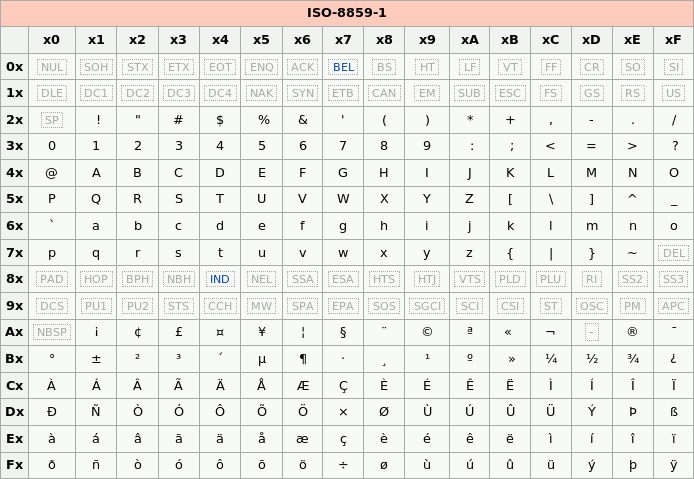
\includegraphics[width=0.9\textwidth]{img/ext-ascii.png}
\end{center}

With this historical and technical background established, we will explore the two main types of modern substitution ciphers: stream ciphers and block ciphers.

	\section{Stream Ciphers}

All of the cryptosystems that we have considered so far fall under the category of {\bf stream ciphers}.  \index{stream cipher} Here is a formal definition.

	\begin{definition}
	A {\bf stream cipher} is a substitution cipher in which the plaintext is encrypted one character (e.g., a letter, bit, or byte) at a time.
	\end{definition}

The following are examples of stream ciphers used since 1900. We won't spend time studying mechanical (e.g. rotor) machines in depth, but are included since they played an important role in cryptographic history.  Stream ciphers are used frequently to encrypt streaming content, such as cell phone calls and internet traffic, because of its speed, simplicity, security, and the flexibility to be used when the length of the plaintext is unknown.

		\subsection{Mechanical Cipher Machines}
		\label{sssec:rotor}

The following are examples of some mechanical cipher machines that were in use from the late 1910s into the 1980s.

		\begin{itemize}
			\item A-21 (Arvid Damm)
			\item Enigma (Arthur Scherbius)
			\item Hebern Machine (Edward Hebern)
			\item KL-51 (NSA)
			\item Lorenz (Germany)
			\item M209-A (Sold to the United States by Boris Hagelin)
			\item PURPLE (97-shiki O-bun in-ji-ki)
		\end{itemize}

	Read \S 2.12 of \cite{tw}

		\subsection{Random and Pseudorandom Number Generators}

So if a one-time pad \index{one-time pad} offers perfect security, an obvious solution would be to somehow generate a random or pseudorandom {\bf keystream}, \index{keystream} a stream of bits to be used as the key, and use a bit-wise addition, modulo $2$, also called a bit-wise {\bf XOR}, \index{XOR} or $\oplus$, to combine it with the plaintext. In this case, the sender and receiver would have to agree on a method to generate a random or pseudorandom sequence of bits and perhaps agree on an additional key (called a {\bf seed}\index{seed}) for the pseudorandom number generator. Before we proceed, it will help to define some terms. (See Chapter 5 of \cite{hac}.)

\begin{definition}
A {\bf random number generator} \index{random number generator} is a device or algorithm which outputs a sequence of statistically independent and unbiased numbers \cite{hac}.
\end{definition}
Typically, the numbers we will generate are binary digits, or bits, so we may alternatively call such a generator a {\bf random bit generator}.

\begin{definition}
A {\bf pseudorandom number generator} \index{pseudorandom number generator} (PRNG) is a deterministic algorithm which inputs a truly random digit sequence and outputs an expanded digit sequence which ``appears" to be random. The input to the PRNG is called the {\bf seed}, \index{seed} while the output of the PRNG is called a {\bf pseudorandom digit sequence} \cite{hac}.
\end{definition}
Again, we will typically be generating a sequence of pseudorandom bits.

The one word in the definition of a PRNG that needs further elaboration in order for this definition to be rigorous is the word {\em appear}. What does it mean to {\em appear} random? There are various statistical tests to measure randomness. (See \S5.4.4 of \cite{hac} or the Statistical Test Suite developed by NIST \cite{nist}.) If a sequence of numbers passes all the tests for randomness in a given test suite, then we say the the sequence {\bf appears} random.

Now just because a number sequence is pseudorandom, doesn't mean that it's secure enough for cryptographic purposes. To this end, we introduce another term.

\begin{definition}
A PRNG is {\bf cryptographically secure} \index{cryptographically secure} if
	\begin{enumerate}
		\item its seed \index{seed} is sufficiently long to make it infeasible to perform a brute-force attack on the PRNG by testing all possible seeds and
		\item given any sequence of digits generated by the PRNG, there is no polynomial-time algorithm that can predict the next digit with any degree of certainty (e.g., with probability greater than $1/2$ for a pseudorandom bit string).
	\end{enumerate}
We may soften this definition somewhat by allowing the sequence of digits in point \#2 to be sufficiently short, specifically, shorter than the length of any intended plaintext or short enough to be stored digitally. It is also common to weaken point \#2 to say that predicting the next bit or digit must be at least as hard as a brute-force attack. We may also add in an assumption that there is sufficient security because the PRNG is based on a mathematical problem that is believed to be solvable in polynomial time.
\end{definition}

Read \S 2.10 of \cite{tw}.


As a note on chronology, the {\bf Blum-Blum-Shub} PRNG \index{Blum-Blum-Shub} (BBS) was published in 1986 and it was motivated by developments in public-key cryptography, notably the RSA \index{RSA} cryptosystem, which we will discuss in Section \ref{ch:pkc}. Its claim of cryptographic security is based on the belief that the {\bf quadratic residuosity problem}\index{quadratic residuosity problem} is computationally difficult when the modulus $n$ is a large composite number. In other words, given $n=pq$, it is believed to be hard to determine if for some $a\in\Z_n$, whether the congruence $x^2 \equiv a \ppmod{n}$ has a solution. This problem is easy if the modulus is prime, so this PRNG relies on the belief that the {\bf integer factorization problem}\index{integer factorization problem} is difficult for large composite integers.


\begin{problem}
\label{prob:lincong1}  [10 points]
Let $x_n = 7 x_{n-1} + 1 \ppmod{10}$ be a linear congruential generator. \index{linear congruential generator} What are all the possible period lengths of this recurrence?
\end{problem}

\begin{problem}
\label{prob:lincong2}  [10 points]
Let $x_n = 7 x_{n-1} + 1 \ppmod{11}$ be a linear congruential generator. \index{linear congruential generator} What are all the possible period lengths of this recurrence?
\end{problem}

\begin{problem}
\label{prob:lincong3}  [10 points]
Based on the results of Problems \ref{prob:lincong1} and \ref{prob:lincong2}, make a conjecture about how the modulus relates to the possible period lengths of a linear congruential generator.\index{linear congruential generator} (You may want to experiment further.)
\end{problem}

\begin{problem}
\label{prob:lincong4}  [10 points]
Suppose that you intercepted a message that used the output of a linear congruential generator \index{linear congruential generator} as the key. Suppose that you determined that the modulus is $17$ and that the first three elements of the keystream were 7, 13, and 9. Based on this information, determine the linear congruential generator that was used and the next three elements of the keystream.
\end{problem}

\begin{problem}
\label{prob:lincong5} [15 points] Suppose that you intercepted a message that used the output of a linear congruential generator \index{linear congruential generator} as the key. Suppose that you determined that the modulus is $997$ and that the first three elements of the keystream were 6, 795, and 978. Based on this information, determine the linear congruential generator that was used and the next three elements of the keystream.
\end{problem}

\begin{problem}
\label{prob:lincong6}  [20 points]
Suppose that you intercepted a message that used the output of a linear congruential generator \index{linear congruential generator} as the key and determined the first ten elements of the keystream: 51, 93, 68, 39, 17, 7, 73, 6, 2, and 9. Based on this information, determine the linear congruential generator that was used and the next three elements of the keystream.
\end{problem}

\begin{problem}  [10 points]
Let $p = 263$ and $q = 283$. If we wanted to use these primes to use BBS as a cryptographically secure PRNG, how many bits could we use with each iteration so generate a cryptographically secure pseudorandom bit stream? Use any seed of your choice to generate 12 pseudorandom bits.
\end{problem}

\begin{problem}
\label{prob:bbs2}  [10 points]
If you wanted to use the Blum-Blum-Shub PRNG as a cryptographically secure PRNG and wanted to use 4 bits with each iteration, how many bits would the modulus $n$ have to have? How many bits would $p$ and $q$ have to have?
\end{problem}

\begin{problem}
\label{prob:bbs3}  [15 points]
As a follow-up to Problem \ref{prob:bbs2}, find primes $p$ and $q$ that would allow you to extract four pseudorandom bits with each iteration. Use the resulting BBS PRNG to generate 32 pseudorandom bits (8 bytes) and encrypt ``{\tt MAT 337!}" using extended-ASCII to encode the eight characters.
\end{problem}

\begin{problem}
\label{prob:bbs4}  [10 points]
Let $p=7$ and $q=11$. What are the possible period lengths of the BBS PRNG?
\end{problem}

\begin{problem}
\label{prob:bbs5}  [10 points]
If $n=pq$ is the modulus of a BBS PRNG, what are some seeds that you would obviously want to avoid?
\end{problem}

\begin{problem}
\label{prob:bbs6} [15 points]
If $n = pq$, and $x_{k+1} = x_k^2\ppmod{n}$, then
$$x_k = \left(x_0^{2^k\ppmod{\lambda(n)}}\right)\ppmod{n} \enspace ,$$
where $\lambda(n) = \lcm((p-1)(q-1))$.
\end{problem}

		\subsection{Other Cryptographically Secure PRNGs}

	The following is a list of other PRNGs that are considered to be cryptographically secure.

		\begin{itemize}
			\item ANSI X9.17 Standard
			\item Blum-Micali
			\item CryptGenRandom
			\item Fortuna
			\item ISAAC
			\item NIST SP 800-90A Standards
			\item Yarrow
		\end{itemize}

\begin{problem} [15 points]
	Do some basic research on one of the PRNGs in the list above. Describe the method, state where and/or how the PRNG is used in practice, and make some brief comments on its security. If it is feasible, generate a cryptographically secure pseudorandom bit sequence by hand or write a program to generate such a sequence.
\end{problem}

		\subsection{Linear Feedback Shift Registers}

		Read \S 2.11 of \cite{tw}.

\begin{problem} [10 points]
\S 2.13 Exercise \#19
\end{problem}

\begin{problem} [10 points]
\S 2.13 Exercise \#20
\end{problem}

\begin{problem} [10 points]
\S 2.13 Exercise \#21
\end{problem}

\begin{problem} [10 points]
\S 2.13 Exercise \#22
\end{problem}

\begin{problem} [15 points]
\S 2.14 Computer Problem \#11
\end{problem}

\begin{problem} [15 points]
\S 2.14 Computer Problem \#12
\end{problem}

\begin{problem} [15 points]
\S 2.14 Computer Problem \#13
\end{problem}

		\subsection{Examples of Modern Stream Ciphers}

	\begin{itemize}
		\item A5/1
		\item ChaCha (Dan Bernstein)
		\item ISAAC (Robert Jenkins, Jr.)
		\item RC4 (Ron Rivest)
		\item Salsa20 (Dan Bernstein)
		\item SEAL (Phillip Rogaway and Don Coppersmith)
		\item Speck (NSA)
		\item Spritz (Ron Rivest)
	\end{itemize}

\begin{problem} [15 points]
	Explore one of the stream ciphers listed above, or any other stream cipher. Include:
	\begin{enumerate}
		\item A mathematical description of the cipher, with pictures if it helps to elucidate the description.
		\item Encrypt your initials using the equivalent non-extended ASCII encoding with the stream cipher and a key of your choice. %(This can be done by hand or by implementing this on a computer.)
		\item Give some examples of applications that use the stream cipher in practice.
		\item Briefly describe the security of the stream cipher. Are there any attacks on the stream cipher that are better than a brute-force attack of the key? If so, are these attacks on the cipher practical or impractical? (This is not intended to be overly technical and should be understood by anyone else in the class.)
	\end{enumerate}
\end{problem}

The disadvantage of just using a stream cipher to encrypt information is that the ciphertext is prone to a {\bf bit-flipping attack}, \index{bit flipping attack}, a form of a man-in-the-middle attack, \index{man-in-the-middle attack} in which an eavesdropper intercepts the message and changes some of the ciphertext. For example, if Eve, the eavesdropper intercepted a message from Alice to Bob that read ``Alice is sending Bob 4 Bitcoins" and she knew the structure of the message, then she could XOR the binary equivalent of ``Bob $\xor$ Eve" in the appropriate location of the message thus changing it to ``Alice is sending Eve 4 Bitcoins" and Eve is suddenly 4 Bitcoins richer! To avoid such an attack, ciphertexts that were encrypted with a stream cipher should include some kind of authentication, such as a message authentication code (MAC) \index{message authentication code}, so that any tampering of the ciphertext would be detected. Man-in-the-middle attacks will be discussed more completely in Section \ref{sssec:mitm} and MACs will be discussed in Section \ref{sssec:mac}.

	\section{Block Ciphers}

In contrast to a stream cipher, {\bf block ciphers} \index{block cipher} encrypt multiple characters, bits, or bytes, called {\bf blocks}, \index{block} at a time. Some classical cryptosystems encrypted blocks of two letters at a time, such as the Playfair Cipher, while modern block ciphers will encrypt plaintext in blocks of 64 or 128 bits, for example. We include two classical cryptosystems here as motivation for modern block ciphers, so with the classical ciphers, the Playfair cipher (\S \ref{sssec:playfair}) and the Hill cipher (\S \ref{sssec:hill}), plaintext and ciphertext will use elements of $\LL$, while subsequent sections will use binary.

		\subsection{The Playfair Cipher} \index{Playfair cipher}
		\label{sssec:playfair}
		Read \S 2.6 of \cite{tw}.

\begin{problem}
\label{prob:playfair}  [10 points]
Encrypt a plaintext of your choice with at least 100 characters with the Playfair cipher using a key your choice. The rest of the class will be challenged later to cryptanalyze the ciphertext.
\end{problem}
\begin{problem}  [15 points]
Recover the plaintext from a peer's ciphertext, which was encrypted using the Playfair cipher in Probem \ref{prob:playfair}.
\end{problem}

		\subsection{The Hill Cipher} \index{Hill cipher}
		\label{sssec:hill}
		Read \S 2.7 of \cite{tw}.

As noted in \cite{tw}, the Hill cipher was not often used, but is notable for being the first to utilize algebraic techniques. The cipher uses distinct encryption and decryption functions (namely, linear transformations) which are inverses of each other. Its downside is that the decryption function is easy to determine from the encryption function because finding the inverse of an invertible matrix is computationally easy.

\begin{problem} [10 points]
\S 2.13 Exercise \#13
\end{problem}

\begin{problem} [10 points]
\S 2.13 Exercise \#14
\end{problem}

\begin{problem} [15 points]
\S 2.13 Exercise \#15
\end{problem}

\begin{problem} [15 points]
\S 2.13 Exercise \#16
\end{problem}

\begin{problem} [15 points]
\S 2.13 Exercise \#17
\end{problem}

\begin{problem} [20 points]
\S 2.13 Exercise \#18
\end{problem}

\begin{problem} [10 points]
\S 2.14 Computer Problem \#10
\end{problem}

\begin{problem}
\label{prob:hill1}  [10 points]
Give an example of an invertible $3\times 3$ matrix with entries in $\Z_{26}$ and find the inverse of the matrix.
\end{problem}

\begin{problem}  [10 points]
How many invertible $2\times 2$ matrices with entries in $\Z_{26}$ are there?
\end{problem}

\begin{problem}  [10 points]
How many invertible $2\times 2$ matrices with entries in $\Z_{37}$ are there?
\end{problem}

\begin{problem}  [10 points]
How many invertible $3\times 3$ matrices with entries in $\Z_{26}$ are there?
\end{problem}

\begin{problem}  [10 points]
How many invertible $3\times 3$ matrices with entries in $\Z_{37}$ are there?
\end{problem}

\begin{problem}  [15 points]
Let $n\in\N$ and let $p$ be a prime. How many invertible $n\times n$ matrices with entries in $\Z_p$ are there?
\end{problem}

\begin{problem}
\label{prob:hill2}  [10 points]
Encrypt a plaintext of your choice with at least 100 characters with the Hill cipher using a key your choice. (This key could be any matrix found in Problem \ref{prob:hill1}. The rest of the class will be challenged later to cryptanalyze the ciphertext.
\end{problem}
\begin{problem}  [10 points if the key is known; 20 points if the key is unknown]
Recover the plaintext from a peer's ciphertext, which was encrypted using the Hill cipher in Problem \ref{prob:hill2}.
\end{problem}


		\subsection{Data Encryption Standard (DES)} \index{DES}\index{Data Encryption Standard}\index{Lucifer}

		Read \S 4.1, 2, 4, and 5 of \cite{tw}.

\paragraph*{Discussion} What are some of the big ideas in the development of DES? What is a Feistel system?

\begin{definition}
	A function $f$ is called a {\bf pseudorandom function} \index{pseudorandom function} if $f$ is an efficient deterministic function whose output cannot be efficiently distinguished from random data.
\end{definition}

\paragraph*{Discussion} Explain why the designers of DES needed a function $f$, as denoted in the description of DES and a simplified DES-type algorithm, that is a pseudorandom function.

\begin{center}
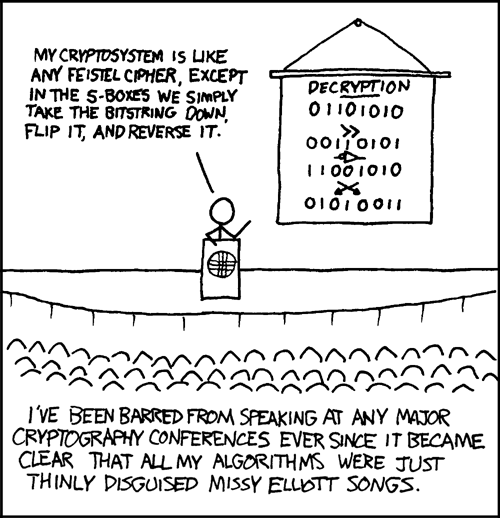
\includegraphics[width=0.5\textwidth]{img/cryptography-xkcd.png}
\end{center}

\begin{problem} [20 points]
Briefly describe the Electronic Codebook (ECB), Cipher Block Chaining (CBC), Cipher Feedback (CFB),  Output Feedback (OFB), and Counter (CTR) modes of operation for block ciphers. What are any strengths and/or weaknesses of each?
\end{problem}
		\subsection{Other Feistel-based Block Ciphers}

		\begin{itemize}
			\item Blowfish
			\item Camellia
			\item CAST-128 and CAST-256
			\item RC5
			\item RC6
			\item Skipjack
			\item TEA (Tiny Encryption Algorithm) and variants
			\item Twofish
			\item 3DES (Triple DES) (\S 4.6 of \cite{tw})
		\end{itemize}

\begin{problem}  [20 points]
Although many block ciphers are proprietary, the description of many block ciphers have been published. Do some basic research on one of the Feistel-based block ciphers above. Answer as many of the following questions as you can.
	\begin{enumerate}
		\item Who created the cipher, what is (are) their affiliation(s), and when was it developed?
		\item What applications use the block cipher?
		\item What size keys does the cipher use and what is the block size that the cipher uses?
		\item Does the cipher make any modifications to the pure Feistel structure?
		\item Describe the pseudorandom function $f$ and any design considerations of the creators.
		\item Briefly state the best known attacks on the cipher. (You will likely come across terminology that we haven't defined yet. That's OK, much of it is quite technical, and later we'll only get a very rough idea of some of the concepts. You're certainly not expected to understand how differential cryptanalysis works, for example.)
	\end{enumerate}
\end{problem}

		\subsection{Other Block Cipher Designs and Components}

		\begin{itemize}
			\item Key Schedule
			\item S-box (substitution box)
			\item P-box (permutation box)
			\item Lai-Massey Scheme
			\begin{itemize}
				\item IDEA
			\end{itemize}
		\end{itemize}

		\subsection{Advanced Encryption Standard (AES)}\index{AES}\index{Advanced Encryption Standard}\index{Rijndael}

		Read Chapter 5 of \cite{tw}.



	\section{Cryptanalysis of Stream and Block Ciphers}

		\subsection{Brute Force Attack}

                \begin{definition}
                  A {\bf brute force attack}\index{brute force attack} on a cryptogram is a cryptanalytic technique in which keys are systematically used to decrypt until the correct key is found.
                \end{definition}

                \begin{problem} [10 points]
                  If a message is encrypted using a 64-bit key, what is an upper bound on the amount of time it would take 1000 computers to crack the ciphertext if each computer can test a million keys per second?
                \end{problem}

                \begin{problem} [10 points]
                  If a message is encrypted using a 128-bit key, what is an upper bound on the amount of time it would take a billion computers to crack the ciphertext if each computer can test a billion keys per second?
                \end{problem}

		\subsection{Known-Plaintext Attacks}

		Read \S 1.1.1 \#2 of \cite{tw}.

		\subsection{Chosen-Plaintext Attacks}

		Read \S 1.1.1 \#3 of \cite{tw}.

		\subsection{Differential Cryptanalysis}

		Read \S 4.3  of \cite{tw}.

		\subsection{Meet-in-the-Middle Attacks}
		\label{sssec:mitm}

		Read \S 4.7 of \cite{tw}.

		\subsection{Black-bag cryptanalysis}

			This isn't mathematical cryptanalysis, but {\bf black-bag cryptanalysis} \index{black-bag cryptanalysis} refers to a generally more practical form of cryptanalysis in which encryption and/or decryption keys or passwords are stolen by any number of means. This may include the following.
		\begin{itemize}
			\item Installation of Trojan horse software on a computer to send passwords to an attacker.
			\item Installation of a keystroke logger to record typing.
			\item Finding a password written on a piece of paper.
			\item Installation of bugs (video and/or audio surveillance) in a room.
			\item Reading electromagnetic transmissions from an electronic device.
			\item Social engineering
		\end{itemize}
		Despite the nontechnical aspects of black-bag methods, it is important to be aware of these forms of cryptanalysis since otherwise unbreakable encryption can be broken if the key is revealed on account of carelessness.

		\subsection{Rubber-hose cryptanalysis}

\begin{center}
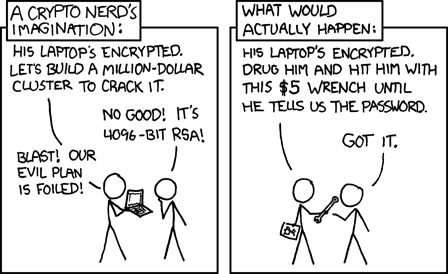
\includegraphics{img/security-xkcd.png}
\end{center}

			As with black-bag methods, {\bf rubber-hose cryptanalysis} \index{rubber-hose cryptanalysis} is not a mathematical technique, but rather any method of recovering encrypted content, a password, or encryption/decryption keys via blackmail, coercion, threats, or torture.


\begin{problem} [15 points]
\S 4.9 Exercise \#1.a.
\end{problem}

\begin{problem} [15 points]
\S 4.9 Exercise \#1.b.
\end{problem}

\begin{problem} [15 points]
\S 4.9 Exercise \#1.c.
\end{problem}

\begin{problem} [10 points]
\S 4.9 Exercise \#2.
\end{problem}

\begin{problem} [15 points]
\S 4.9 Exercise \#3.
\end{problem}

\begin{problem} [15 points]
\S 4.9 Exercise \#4.
\end{problem}

\begin{problem} [15 points]
\S 4.9 Exercise \#5.
\end{problem}

\begin{problem} [15 points]
\S 4.9 Exercise \#6.
\end{problem}

\begin{problem} [15 points]
\S 4.9 Exercise \#7.
\end{problem}

\begin{problem} [10 points]
\S 4.9 Exercise \#8.
\end{problem}

\begin{problem} [15 points]
\S 4.9 Exercise \#9.
\end{problem}

\begin{problem} [10 points]
\S 4.9 Exercise \#10.
\end{problem}

\begin{problem} [10 points]
\S 4.9 Exercise \#11.
\end{problem}

\begin{problem} [15 points]
\S 4.10 Computer Problem \#1.a and 1.b.
\end{problem}

\begin{problem} [10 points]
\S 4.10 Computer Problem \#1.c.
\end{problem}

\begin{problem} [10 points]
\S 4.10 Computer Problem \#1.d.
\end{problem}

\begin{problem} [10 points]
\S 4.10 Computer Problem \#2.
\end{problem}

\begin{problem} [10 points]
Explore a topic that came out of a class discussion or solve a problem inspired by the content of this chapter.
\end{problem}

\chapter{Mathematical Interlude}
\label{ch:math}
	\section{Hash Functions}

\begin{definition}
A {\bf hash function} \index{hash function} $h:\{0,1\}^* \to \N$ is a function that maps an arbitrarily long input to an integer of some fixed size.
\end{definition}

Hash functions are commonly used in computer science primarily to store data in large arrays in a way that makes the data quick and easy to store and retrieve. Hash functions have different uses in cryptography, but require two additional properties in order to make them useful for cryptographic purposes.

\begin{definition}
A {\bf cryptographically secure hash function} is a hash function $h$ such that
\begin{enumerate}
\item $h$ is {\bf one-way}\index{one-way}, that is, given some element $r\in\N$ in the range of $h$, it is computationally infeasible to compute an input $m$ such that $h(m)=r$; and
\item it is computationally infeasible to find a {\bf collision}, that is, two distinct elements $m_1$ and $m_2$ in the domain of $h$ such that $h(m_1) = h(m_2)$.
\end{enumerate}
\end{definition}

The following are examples of hash functions that have once been or are considered to be cryptographically secure.

	\begin{itemize}
		\item MD5 (Ron Rivest)
		\item MD6 (Ron Rivest et al.)
		\item SHA-1 (NSA)
		\item SHA-2 (NSA)
		\item SHA-3 / Keccak (Guido Bertoni, Joan Daemen, Gilles Van Assche, and Micha\"{e}l Peeters
	\end{itemize}

	Read \S 8.1-8.3, 8.7 of \cite{tw}.

	\section{The Birthday Problem}

	The {\bf birthday problem}\index{birthday problem} is a standard cryptanalytic technique that is used to attack hash functions. It is also at the heart of an algorithm called Pollard's Rho algorithm for factoring integers and computing discrete logarithms. (\S 8.4.1 of \cite{tw})

	Read \S 8.4 of \cite{tw}.

\begin{problem} (10 points)
	\S 8.8 Exercise \#1
\end{problem}

\begin{problem} (10 points)
	\S 8.8 Exercise \#3
\end{problem}

\begin{problem} (20 points)
	\S 8.8 Exercise \#5
\end{problem}

\begin{problem} (10 points)
	\S 8.8 Exercise \#6
\end{problem}

\begin{problem} (5 points)
	\S 8.8 Exercise \#8
\end{problem}

\begin{problem} (10 points)
	\S 8.8 Exercise \#9
\end{problem}

\begin{problem} (15 points)
	\S 8.8 Exercise \#10
\end{problem}

\begin{problem} (20 points)
	\S 8.8 Exercise \#11
\end{problem}

\begin{problem} (10 points)
	\S 8.9 Computer Problem \#1
\end{problem}

\begin{problem} (10 points)
	\S 8.9 Computer Problem \#2
\end{problem}

	%\section{Computational Complexity}

	\section{Group Theory}
	\label{ssec-groups}

\begin{definition}
A {\bf group}\index{group} is a nonempty set $G$, together with a binary operation, $*$, such that the following four axioms hold.
\begin{enumerate}
	\item $G$ is {\bf closed} under the operation $*$. That is, for all $a, b\in G$, $a*b \in G$.
	\item The operation $*$ is {\bf associative} in $G$. That is, for all $a, b, c\in G$, $(a*b)*c = a*(b*c)$.
	\item $G$ possesses an {\bf identity element}, $e$. That is, for all $a \in G$, $e*a = a*e = a$.
	\item Every element $a\in G$ has an {\bf inverse} in $G$. That is, for all $a\in G$, there is some element $a^{-1}\in G$ such that $a*a^{-1} = a^{-1}*a = e$. (If * is an additive operation, then the inverse of $a$ is typically denoted $-a$.
\end{enumerate}
\end{definition}
Notice that groups need not be commutative. Such groups have a special name.
\begin{definition}
	If any two elements $a, b\in G$ commute under the operation $*$, that is, if $a*b = b*a$, for all $a,b\in G$, then $G$ is called an {\bf abelian}\index{abelian} group.
\end{definition}

\begin{problem}  [10 points]
	Show that the set $\Z_n$ is an abelian group under the operation of addition modulo $n$.
\end{problem}
\begin{problem}  [10 points]
	Show that the set $\Z_p^* = \{1, \ldots, p-1\}$ is an abelian group under the operation of multiplication modulo $p$.
\end{problem}

\begin{problem}  [10 points]
	Show that the set $\Z_n^* = \{1\le a <n \mid \gcd(a, n)=1\}$ is an abelian group under the operation of multiplication modulo $n$.
\end{problem}

\begin{definition}
	The number of elements of a group $G$ is called its {\bf order} and is denoted $|G|$.
\end{definition}

\begin{definition}
{\bf Euler's phi (or totient) function}\index{phi function}\index{totient function} is defined to be $\varphi(n) = |\Z_n^*| = |\{1\le a <n \mid \gcd(a, n)=1\}|$.
\end{definition}

\begin{definition}
If $G$ is a group, $H\subseteq G$, and $H$ is a group, then $H$ is called a {\bf subgroup}\index{subgroup} of $G$ and we write $H \le G$.
\end{definition}

\begin{definition}
	The subgroup of $G$ {\bf generated} by $g\in G$ is the set $\<g\> = \{g^n \mid n\in\Z\}$. If there is some $g\in G$ such that $\<g\> = G$, then $G$ is called a {\bf cyclic} group and $g$ is called a {\bf generator} of $G$.
\end{definition}

\begin{definition}
	If $p$ is a prime and $r\in\Z_p^*$ such that $\<r\>=\Z_p^*$, then $r$ is called a {\bf primitive root}\index{primitive root} modulo $p$.
\end{definition}

\begin{problem}  [15 points]
Prove that all cyclic groups are abelian.
\end{problem}

\begin{problem}  [10 points]
Find a generator of $\Z_{97}^*$.
\end{problem}

\begin{theorem}[Lagrange]
\label{thm:lagrange}
If $H\le G$, then $|H|\mid |G|$.
\end{theorem}

\begin{problem}[15 points]
Prove Lagrange's Theorem (Theorem \ref{thm:lagrange}).
\end{problem}


	\section{Modular Exponentiation}

	Read \S 3.5 of \cite {tw}.

	In many situations, we must perform some exponentiation, say $a^x \ppmod{m}$, for some $m\in\N$, $a\in\Z_m$, and $x\in\Z$. If $|x|$ is very large, then we certainly do not want to multiply $a$ (or its inverse) by itself $|x|$ times. A common approach to compute this number is {\bf binary exponentiation}\index{binary exponentiation}. It is best illustrated with an example.

{\bf Example.} Compute: $2^{42} \ppmod{97}$.

We compute this using the binary representation of the exponent and make successive squarings.

$2^{42} = 2^{32 + 8 + 2} = (2^{32})(2^8)(2^2).$
\begin{center}
\begin{tabular}{|c|c|c|}
\hline
$k$ & $2^k$ & $2^{2^k} \ppmod{97}$\\
\hline
0 & 1 & 2\\
1 & 2 & $2^2 = 4$\\
2 & 4 & $4^2 = 16$\\
3 & 8 & $16^2 \equiv 62 \ppmod{97}$\\
4 & 16 & $62^2 \equiv 61 \ppmod{97}$\\
5 & 32 & $61^2 \equiv 35 \ppmod{97}$\\
\hline
\end{tabular}
\end{center}
So
$$2^{42} = (2^{32})(2^8)(2^2) \equiv 35\cdot 62 \cdot 4 \equiv 47 \ppmod{97} \enspace .$$

\begin{problem} [10 points]
Compute $3^{409} \ppmod{997}$.
\end{problem}

\begin{problem}[10 points]
Compute $3^{-251}\ppmod{997}$.
\end{problem}

\begin{problem}[15 points]
What is the {\bf non-adjacent form} (NAF) of an integer and how can it be used to improve binary exponentiation?
\end{problem}

		\paragraph*{Fermat's Little Theorem}

		\begin{theorem}[Fermat's Little Theorem]
			If $p$ is a prime and $a\in \Z$ such that $p\nmid a$, then $a^{p-1} \equiv 1 \ppmod{p}$.
		\end{theorem}

		\begin{problem}  [10 points]
			Prove Fermat's Little Theorem.
		\end{problem}

		\begin{problem} [15 points]
			In Section \ref{ssec-groups}, we defined a primitive root of a prime $p$ as an integer $r$ such that $\<r\>=\Z_p^*$. Describe a method to determine whether or not a given $r\in\Z$ is a primitive root modulo $p$ that is more efficient than a brute-force search.
		\end{problem}

		\paragraph*{Euler's Theorem}

		\begin{theorem}[Euler]
			If $a,n\in\Z$ such that $\gcd(a,n)=1$, then $a^{\varphi(n)} \equiv 1 \ppmod{n}$.
		\end{theorem}

		\begin{problem}  [10 points]
			Prove Euler's Theorem.
		\end{problem}

		\begin{problem}[10 points]
			\S3.13 \#2 of \cite{tw}.
		\end{problem}

		\begin{problem}[10 points]
			\S3.13 \#11 of \cite{tw}.
		\end{problem}

		\begin{problem}[10 points]
			\S3.13 \#12 of \cite{tw}.
		\end{problem}

		\begin{problem}[10 points]
			\S3.13 \#13 of \cite{tw}.
		\end{problem}

		\begin{problem}[10 points]
			\S3.13 \#15 of \cite{tw}.
		\end{problem}

		\begin{problem}[10 points]
			\S3.13 \#16 of \cite{tw}.
		\end{problem}

		\begin{problem}[10 points]
			\S3.13 \#17 of \cite{tw}.
		\end{problem}

		\begin{problem}[20 points]
			\S3.13 \#20 of \cite{tw}.
		\end{problem}

		\begin{problem}[20 points]
			\S3.13 \#21 of \cite{tw}.
		\end{problem}

		\begin{problem}[10 points]
			\S3.14 \#3 of \cite{tw}.
		\end{problem}

		\begin{problem}[10 points]
			\S3.14 \#7 of \cite{tw}.
		\end{problem}

		\begin{problem}[10 points]
			\S3.14 \#9 of \cite{tw}.
		\end{problem}

		\paragraph*{Carmichael Function}

\begin{definition}
	The {\bf Carmichael function}, $\lambda:\N\to\N$, on input $n$ is the smallest positive integer $\lambda(n)$ such that $a^{\lambda(n)} \equiv 1\ppmod{n}$ for every $a$ that is relatively prime to $n$.
\end{definition}


		\paragraph*{Quadratic Residues and Modular Square Roots}

		Stretching the concept of modular exponentiation, we can consider modular square roots. This has some interesting cryptographic applications that we will encounter later. Let's establish some terminology.


\begin{definition}
Let $n\in\Z$. An integer $a$ is said to be a {\bf quadratic residue}\index{quadratic residue} modulo $n$ if there is some $x\in\Z$ such that $x^2 \equiv a \ppmod{n}$. If $a$ is a quadratic residue modulo $n$ and $x^2 \equiv a \ppmod{n}$, then $x$ is a {\bf square root} of $a$ modulo $n$ and we can write $x \equiv \sqrt{a} \ppmod{n}$.

For the case that $n=p$ is an odd prime, the {\bf Legendre symbol}\index{Legendre symbol} is defined:

$$\left(\frac{a}{p}\right)  = \left\{\begin{array}{rl}
-1 & \mbox{ if } a \mbox{ is not a quadratic residue modulo } p\\
 1 & \mbox{ if } a \mbox{ is a quadratic residue modulo } p\\
 0 & \mbox{ if } p\mid a.
\end{array}\right.$$
\end{definition}



\begin{theorem}[Euler's Criterion]
If $p$ is an odd prime and $a\in\Z$ such that $\left(\frac{a}{p}\right)=1$, then
$$a^{\frac{p-1}{2}} \equiv \left(\frac{a}{p}\right) \ppmod{p}.$$
\end{theorem}

\begin{problem}[15 points]
Prove Euler's Criterion.
\end{problem}

\begin{problem}[15 points]
Prove that if $p$ is an odd prime and $p\nmid ab$, then
$$\left(\frac{ab}{p}\right) = \left(\frac{a}{p}\right)\left(\frac{b}{p}\right).$$
\end{problem}

\begin{problem}[10 points]
If $p$ is an odd prime, determine $\left(\frac{-1}{p}\right)$.
\end{problem}

\begin{problem}[10 points]
If $p$ is an odd prime and $a\equiv b \ppmod{p}$, then $\left(\frac{a}{p}\right)=\left(\frac{b}{p}\right)$.
\end{problem}

A much more efficient way to determine whether a given integer is a quadratic residue modulo an odd prime is to apply the Law of Quadratic Reciprocity.

\begin{theorem}[Quadratic Reciprocity]
Let $p$ and $q$ be odd primes.
$$\left(\frac{2}{p}\right)=1 \mbox{ if and only if } p\equiv 1,7 \ppmod{8}$$
$$\left(\frac{q}{p}\right) = \left\{ \begin{array}{rl}
-\left(\frac{p}{q}\right) & \mbox{ if } p,q\equiv 3\ppmod{4}\\
 \left(\frac{p}{q}\right) & \mbox{ otherwise. }
\end{array}\right.$$
\end{theorem}


\begin{problem}[10 points]
Find all quadratic residues modulo 19.
\end{problem}

Now we turn to actually computing modular square roots. For primes congruent to 1 modulo 4, the process can be a little involved. Fortunately, it is straightforward for all other primes, and these are the kinds of primes that cryptographers are most interested in.

\begin{theorem}
\label{thm:sqrtmodp}
If $p\equiv 3 \ppmod{4}$ is prime and $\left(\frac{a}{p}\right)=1$, then $\sqrt{a} \equiv \pm a^{(p+1)/4}\ppmod{p}$.
\end{theorem}

\begin{problem}[10 points]
Determine $\pm\sqrt{31}\ppmod{43}$.
\end{problem}

\begin{problem}[15 points]
Prove Theorem \ref{thm:sqrtmodp}.
\end{problem}

\begin{problem}[10 points]
Show that if $p$ is an odd prime and $a\in\Z$ such that $\left(\frac{a}{p}\right)=1$, then $x^2 \equiv a \ppmod{p}$ has two distinct solutions in $\Z_p^*$. (In other words, $a$ has two square roots modulo $p$.)
\end{problem}

Now if $n=pq$ is a product of primes, then we can compute square roots modulo $n$.
\begin{theorem}
\label{thm:sqrtmodn}
Let $n=pq$ be a product of distinct primes and let $a\in\Z$ such that $\left(\frac{a}{p}\right)=\left(\frac{a}{q}\right)=1$. Then $a$ is a quadratic residue modulo $n$ and
$$\sqrt{a} \equiv r_1dq + r_2cp \ppmod{n}\enspace ,$$
where $r_1 \equiv \sqrt{a} \ppmod{p}$, $r_2 \equiv \sqrt{a} \ppmod{q}$, and $c,d\in\Z$ such that $cp+dq = 1$.
\end{theorem}
Notice that since $p=q$, $\gcd(p,q)=1$, so there do exist $c,d\in\Z$ such that $cp+dq=1$.

\begin{problem}[15 points]
Prove Theorem \ref{thm:sqrtmodn}.
\end{problem}

\begin{problem}[10 points]
Find a quadratic residue modulo 77 and compute its square root modulo 77.
\end{problem}

\begin{problem}[15 points]
Show that if $p$ and $q$ are distinct odd primes, $n=pq$ and $a\in\Z$ such that $\left(\frac{a}{p}\right)=\left(\frac{a}{q}\right)=1$, then $x^2 \equiv a \ppmod{n}$ has four distinct solutions in $\Z_p^*$. (In other words, $a$ has four square roots modulo $n$.)
\end{problem}



	\section{Discrete Logarithms}

	\begin{definition}
		Let $G$ be a group, $g\in G$, and $h\in\<g\>$. That is, there is some $x\in\N_0$ such that $g^x = h$. The integer $x$ is called the {\bf discrete logarithm} of $h$ in $\<g\>$.
		If $p$ is prime and $g\in\Z_p^*$ such that $\<g\> = \Z_p^*$, then for some $h\in\Z_p^*$, the integer $x\in\N_0$ such that $g^x \equiv h \ppmod{p}$ is the discrete logarithm of $h$ to base $g$ modulo $p$.
	\end{definition}

Read \S 7.1 and 7.2 in \cite{tw}.

\begin{problem}[10 points]
	Compute $\log_2(3) \pmod{13}$.
	Compute $\log_2(11) \ppmod{13}$.
\end{problem}

\begin{problem}[10 points]
	Use Pohlig-Hellman to compute $\log_2(14) \ppmod{19}$.
\end{problem}

\begin{problem}[15 points]
	\S 7.6 \#5 of \cite {tw}
\end{problem}

\begin{problem}[15 points]
	\S 7.6 \#6 of \cite {tw}
\end{problem}

\begin{problem}[15 points]
	\S 7.6 \#7 of \cite {tw}
\end{problem}

\begin{problem}[10 points]
	\S 7.6 \#8 of \cite {tw}
\end{problem}

\begin{problem}[10 points]
	\S 7.7 \#2 of \cite {tw}
\end{problem}

\begin{problem}[5 points]
	\S 7.7 \#3 of \cite {tw}
\end{problem}

\begin{problem}[10 points]
	\S 7.7 \#4 of \cite {tw}
\end{problem}


	\section{Primality Testing}

Read \S6.3 of \cite{tw}.

\begin{problem}[10 points]
	\S 6.9 \#13 of \cite {tw}
\end{problem}

\begin{problem}[15 points]
	Describe a method to test whether a given $n\in\N$ is composite or possibly prime.
\end{problem}

	\section{Integer Factorization}

Read \S6.4 of \cite{tw}.

\begin{problem}[10 points]
	\S 6.8 \#12 of \cite {tw}
\end{problem}

\begin{problem}[10 points]
	\S 6.8 \#13 of \cite {tw}
\end{problem}

\begin{problem}[10 points]
	\S 6.9 \#4 of \cite {tw}
\end{problem}

\begin{problem}[10 points]
	\S 6.9 \#5 of \cite {tw}
\end{problem}

\begin{problem}[10 points]
	\S 6.9 \#6 of \cite {tw}
\end{problem}

\begin{problem}[10 points]
	\S 6.9 \#8 of \cite {tw}
\end{problem}

\begin{problem}[10 points]
	\S 6.9 \#9 of \cite {tw}
\end{problem}

\begin{problem}[10 points]
	\S 6.9 \#10 of \cite {tw}
\end{problem}

\begin{problem}[10 points]
	\S 6.9 \#12 of \cite {tw}
\end{problem}

	\section{Finite Fields}

We learned about Linear Feedback Shift Registers earlier. To get a deeper understanding into why they function the way they do, we turn to finite fields. This section is also applied to many areas of cryptography and coding theory.

Read \S 3.11 of \cite{tw}.

	\begin{definition}
          A {\bf field}\index{field} is a nonempty set $K$, together with two commutative binary operations, addition and multiplication, having the following properties.
          \begin{itemize}
            \item $K$ is an abelian group with identity $0$ under addition.
            \item $K^* = K\setminus\{0\}$ is an abelian group with identity $1$ under multiplication.
            \item $a(b+c) = ab + ac$ for all $a, b, c \in K$.
          \end{itemize}
        \end{definition}

        \begin{problem} [10 points]
          Give three examples of fields of infinite order (cardinality).
        \end{problem}

        \begin{problem} [10 points]
          Show that $\Z_p = \{0, 1, \ldots, p-1\}$ is a field if and only if $p$ is prime. ($\Z_p$ will often be denoted $\F_p$ or $GF(p)$.)
        \end{problem}

        \begin{theorem}
          If $K$ is a finite field, then $|K| = p^n$, for some prime $p$ and $n\in\N$. $K \isom \F_p[x]/\<f(x)\>$, where $f(x)\in\F_p[x]$ is irreducible.
        \end{theorem}

        \begin{problem} [20 points]
          Show that if $p$ is a prime and $f(x)\in\F_p[x]$ is irreducible, then $\F_p[x]/\<f(x)\>$ is a field of order $p^n$.
        \end{problem}

	\begin{problem}[15 points]
		\S3.13 \#33 of \cite{tw}.
	\end{problem}

	\begin{problem}[10 points]
		\S3.13 \#34 of \cite{tw}.
	\end{problem}

        \begin{problem} [15 points]
          Let $p = 2$. Find an irreducible cubic polynomial over $\F_2$. Describe the elements of $\F_{2^3}$.
        \end{problem}

\chapter{Public-Key Cryptography}
\label{ch:pkc}
	\section{The Concept}

	Read \S 6.7 of \cite{tw}.

The concept of Diffie-Hellman Key Exchange can be understood even by elementary school children with an activity called ``Chocolate key cryptography," using M\&Ms \cite{mandm}.

% Activity - Chocolate Key Cryptography
%Set-up: Two empty cans with plastic lids. Each can represents an encryption/decryption key.
%Cut a pair of crossed slits about 1/2 inch long in each lid.
%``Alice" and ``Bob" each get a can.
%``Alice" and ``Bob" put as many M&M's of whatever color as they want into their respective cans.
%Nobody in possession of a can is allowed to open the can, but can ``copy" the can.
%``Alice" and ``Bob" give their can to each other and each put their identical M&Ms into the can.
%Now Alice and Bob's cans contain the same number and color of M&Ms.


	\section{Diffie-Hellman-(Merkle) Key Exchange}

Read \S 7.4 of \cite{tw}.

\begin{problem}[15 points]
	Describe how to extend the Diffie-Hellman Key Exchange for three people to share a common secret key.
\end{problem}

\begin{problem}[15 points]
	Describe how to extend the Diffie-Hellman Key Exchange for $n$ people to share a common secret key.
\end{problem}

\begin{problem}[15 points]
	\S 7.6 \#10 of \cite {tw}
\end{problem}

	\section{Kid Krypto}

	Kid Krypto \index{Kid Krypto} is a warm-up to the RSA public-key cryptosystem. Many of the concepts are identical, but the mathematics of Kid Krypto is a little more basic.

If Bobby would like to receive a secret message from his friends, he first chooses any four positive integers that only he will know: $a, b, A$, and $B$. Then he computes
\begin{align*}
M &= ab-1 \\
e &= AM+a \\
d &= BM+b \\
n &= \frac{ed-1}{M}
\end{align*}
Bobby tells everyone the numbers $e$ (for encryption) and $n$. To send a plaintext message $m\in\Z_n$, the sender computes
$$ c = em \ppmod n \enspace .$$
To decipher the ciphertext $c$, Bobby computes
$$ dc \ppmod{n} \enspace .$$

\begin{problem}  [10 points]
Let $a = 47$, $b = 22$, $A=11$, and $B=5$. Compute $M, e, d,$ and $n$.
	\begin{enumerate}
		\item Encode the plaintext message $m = 2020$ using $e$ and $n$ above. (Check that $dc \ppmod{n} = m$.)
%16414
		\item Decode the encrypted message $c = 43155$. (Check that $em \ppmod{n} = c$.)
%1234
	\end{enumerate}
\end{problem}
\begin{problem}
\label{prob:kk}  [10 points]
Bobby announces his public key: $n = 17239722505$, $e = 25540219$. Alice sends him the encrypted message $c = 7218695996$. What is Alice's message?
%314159
\end{problem}

\begin{problem}   [10 points]
Explain why Kid Krypto works; that is, how do you know that $m = dc \ppmod{n}$?
\end{problem}
\begin{problem}  [10 points]
Is Kid Krypto secure? Discuss its strengths and weaknesses.
\end{problem}

\begin{problem}  [10 points]
Using the same values of $n$ and $e$ from Problem \ref{prob:kk}, decode the value of $m$ from the intercepted message $c =6599969821$. The number you've found is not just a randomly chosen number. It corresponds to an English word or phrase. What is the word and how is it derived from $m$?
\end{problem}
	\section{RSA}

Read \S 6.1 (6.2 is optional) of \cite {tw}.

\begin{problem}[10 points]
	\S 6.8 \#1 of \cite {tw}
\end{problem}

\begin{problem}[10 points]
	\S 6.8 \#2 of \cite {tw}
\end{problem}

\begin{problem}[10 points]
	\S 6.8 \#3 of \cite {tw}
\end{problem}

\begin{problem}[10 points]
	\S 6.8 \#4 of \cite {tw}
\end{problem}

\begin{problem}[10 points]
	\S 6.8 \#5 of \cite {tw}
\end{problem}

\begin{problem}[10 points]
	\S 6.8 \#6 of \cite {tw}
\end{problem}

\begin{problem}[15 points]
	\S 6.8 \#7 of \cite {tw}
\end{problem}

\begin{problem}[10 points]
	\S 6.8 \#8 of \cite {tw}
\end{problem}

\begin{problem}[20 points]
	\S 6.8 \#9 of \cite {tw}
\end{problem}

\begin{problem}[15 points]
	\S 6.8 \#11 of \cite {tw}
\end{problem}

\begin{problem}[15 points]
	\S 6.8 \#16 of \cite {tw}
\end{problem}

\begin{problem}[10 points]
	\S 6.8 \#17 of \cite {tw}
\end{problem}

\begin{problem}[15 points]
	\S 6.8 \#19 of \cite {tw}
\end{problem}

\begin{problem}[10 points]
	\S 6.8 \#22 of \cite {tw}
\end{problem}

\begin{problem}[5 points]
	\S 6.9 \#1 of \cite {tw}
\end{problem}

\begin{problem}[10 points]
	\S 6.9 \#2 of \cite {tw}
\end{problem}

\begin{problem}[10 points]
	\S 6.9 \#3 of \cite {tw}
\end{problem}

\begin{problem}[20 points]
	\S 7.6 \#12 of \cite {tw}
\end{problem}

	\section{ElGamal}

	Read \S 7.5 of \cite{tw}.

\begin{problem}[10 points]
	\S 7.6 \#11 of \cite {tw}
\end{problem}

	\section{Elliptic Curve Cryptography}

	There are special groups arising from curves called {\bf elliptic curves}\index{elliptic curve} that are ubiquitous in cryptography today. An understanding of group theory and finite fields will facilitate understanding these objects more fully and will allow for problems to be solved much more easily.

	Read Chapter 16 of \cite{tw}.

\begin{problem}[15 points]
	\S 16.7 \#2 of \cite {tw}
\end{problem}

\begin{problem}[10 points]
	\S 16.7 \#3 of \cite {tw}
\end{problem}

\begin{problem}[10 points]
	\S 16.7 \#4 of \cite {tw}
\end{problem}

\begin{problem}[10 points]
	\S 16.7 \#5 of \cite {tw}
\end{problem}

\begin{problem}[15 points]
	\S 16.7 \#6 of \cite {tw}
\end{problem}

\begin{problem}[15 points]
	\S 16.7 \#7 of \cite {tw}
\end{problem}

\begin{problem}[10 points]
	\S 16.7 \#8 of \cite {tw}
\end{problem}

\begin{problem}[20 points]
	\S 16.7 \#9 of \cite {tw}
\end{problem}

\begin{problem}[10 points]
	\S 16.7 \#10 of \cite {tw}
\end{problem}

\begin{problem}[15 points]
	\S 16.7 \#11 of \cite {tw}
\end{problem}

\begin{problem}[15 points]
	\S 16.7 \#12 of \cite {tw}
\end{problem}

\begin{problem}[15 points]
	\S 16.7 \#13 of \cite {tw}
\end{problem}

\begin{problem}[20 points]
	\S 16.7 \#14 of \cite {tw}
\end{problem}

\begin{problem}[20 points]
	\S 16.7 \#15 of \cite {tw}
\end{problem}

\begin{problem}[15 points]
	\S 16.7 \#16 of \cite {tw}
\end{problem}

\begin{problem}[15 points]
	\S 16.7 \#17 of \cite {tw}
\end{problem}

\begin{problem}[15 points]
	\S 16.7 \#18 of \cite {tw}
\end{problem}

\begin{problem}[15 points]
	\S 16.7 \#19 of \cite {tw}
\end{problem}

\begin{problem}[20 points]
	\S 16.7 \#20 of \cite {tw}
\end{problem}

\begin{problem}[15 points]
	\S 16.8 \#1 of \cite {tw}
\end{problem}

\begin{problem}[10 points]
	\S 16.8 \#2 of \cite {tw}
\end{problem}

\begin{problem}[20 points]
	\S 16.8 \#3 of \cite {tw}
\end{problem}

\begin{problem}[15 points]
	\S 16.8 \#4 of \cite {tw}
\end{problem}

\begin{problem}[10 points]
	\S 16.8 \#5 of \cite {tw}
\end{problem}

\begin{problem}[20 points]
	Give the mathematical details of Curve25519 and explain the difference in the representation of this curve from the standard Weierstrass form of an elliptic curve. Who created the curve, what were the design considerations, and why is this curve used in so many applications today?
\end{problem}

\chapter{Cryptographic Protocols}
\label{ch:protocols}
	\section{Zero-Knowledge Proofs}

Read \S 14.1 of \cite{tw}.

\begin{problem}[10 points]
	\S 14.3 \#1 of \cite {tw}
\end{problem}

\begin{problem}[15 points]
	\S 14.3 \#2[a,b] of \cite {tw}
\end{problem}

\begin{problem}[10 points]
	\S 14.3 \#2[c] of \cite {tw}
\end{problem}

\begin{problem}[10 points]
	\S 14.3 \#3[a] of \cite {tw}
\end{problem}

\begin{problem}[15 points]
	\S 14.3 \#3[b, c] of \cite {tw}
\end{problem}

\begin{problem}[15 points]
	\S 14.3 \#4[a, b] of \cite {tw}
\end{problem}

\begin{problem}[15 points]
	\S 14.3 \#4[c, d] of \cite {tw}
\end{problem}

\begin{problem}[15 points]
	\S 14.3 \#5 of \cite {tw}
\end{problem}

\begin{problem}[15 points]
	\S 14.3 \#6 of \cite {tw}
\end{problem}

	\section{Identification Schemes and Authentication}
Read \S 14.2 of \cite{tw}.

	%aka Authentication
	\subsection{Message Authentication Codes}
	\label{sssec:mac}

\begin{definition}
A {\bf message authentication code (MAC)} is data transmitted with a message that verifies that the message came from the stated sender (authentication) and that the data has not been altered during the transmission (integrity).
\end{definition}

	The following are examples of MAC algorithms and frameworks
	\begin{itemize}
		\item CBC-MAC
		\item Checksum (using a hash function), e.g. md5sum, sha1sum
		\item HMAC
		\item Poly1305 and Poly1305-AES (Dan Bernstein)
	\end{itemize}


\begin{problem}  [15 points]

	\begin{enumerate}
		\item Who created the MAC, what is (are) their affiliation(s), and when was it developed?
		\item How is the MAC or MAC framework used?
		\item Discuss the details of the MAC or framework. Pictures help.
		\item Discuss the security of the MAC or MAC framework.
	\end{enumerate}
\end{problem}


	\section{Digital Signatures}
	%Also Blind signatures

	Read Chapter 9 of \cite{tw}.

	Another signature scheme is Rabin's Signature Algorithm. Suppose that Alice sends a message $M$ to Bob. She wants to sign the message to prove to Bob that she alone sent the message.

	\begin{enumerate}
		\item Alice chooses two distinct primes $p,q\equiv 3\ppmod{4}$ and keeps these two primes private. (Ideally, $p$ and $q$ are {\bf safe} primes, i.e. primes such that $p=2r+1$ and $q = 2s+1$, where $r$ and $s$ are prime.)
		\item Alice and Bob agree on a cryptographically secure hash function, $h$.
		\item Alice chooses a random padding $u$ and concatenates $m=M||u$.
		\item If $h(m)$ is not a quadratic residue modulo $p$ and modulo $q$, go back to Step 3.
		\item Alice computes $s = \sqrt{h(m)}$ and sends $s$ and $m$ to Bob.
		\item Bob verifies that $s^2 \equiv h(m) \ppmod{n}$.
	\end{enumerate}


\begin{problem}[10 points]
	Why is Rabin's Signature Algorithm secure?
\end{problem}

\begin{problem}[10 points]
	Choose two 3-digit safe primes and sign the message $M=1618$. Use a 1-digit pad and skip the use of a hash function.
\end{problem}

\begin{problem}[15 points]
	\S 9.6 \#1 of \cite {tw}
\end{problem}

\begin{problem}[15 points]
	\S 9.6 \#2 of \cite {tw}
\end{problem}

\begin{problem}[10 points]
	\S 9.6 \#3 of \cite {tw}
\end{problem}

\begin{problem}[10 points]
	\S 9.6 \#4[a] of \cite {tw}
\end{problem}

\begin{problem}[10 points]
	\S 9.6 \#4[b] of \cite {tw}
\end{problem}

\begin{problem}[10 points]
	\S 9.6 \#4[c] of \cite {tw}
\end{problem}

\begin{problem}[15 points]
	\S 9.6 \#5 of \cite {tw}
\end{problem}

\begin{problem}[10 points]
	\S 9.6 \#6 of \cite {tw}
\end{problem}

\begin{problem}[10 points]
	\S 9.6 \#7 of \cite {tw}
\end{problem}

\begin{problem}[15 points]
	\S 9.6 \#8 of \cite {tw}
\end{problem}

\begin{problem}[10 points]
	\S 9.7 \#1 of \cite {tw}
\end{problem}

\begin{problem}[10 points]
	\S 9.7 \#2 of \cite {tw}
\end{problem}

\begin{problem}[10 points]
	\S 9.7 \#3 of \cite {tw}
\end{problem}

	\section{Secret Sharing and Threshold Schemes}

Read Chapter 12 of \cite{tw}.
	%Activity: encrypt a password as the constant term of a linear congruence. Give each student a point on the line. Have them determine the password.
	% Have a "spy" with a fake point. Figure out who the spy is.

\begin{problem}[10 points]
	Let $p$ be the smallest prime greater than $2^{20}$ and let $q(x) = ax^2+bx+c \ppmod{p}$ be a quadratic polynomial modulo $p$. A PIN has been encoded as the constant term, $c$, of $q(x)$. Alice, Bob, and Charlie have been given the points of the curve $y=q(x)$: $(984544, 900317)$, $(248781, 118521)$, and $741200, 198787)$, respectively. Recover the PIN.
% 314531
\end{problem}

\begin{problem}[10 points]
	\S 12.3 \#1 of \cite {tw}
\end{problem}

\begin{problem}[10 points]
	\S 12.3 \#2 of \cite {tw}
\end{problem}

\begin{problem}[5 points]
	\S 12.3 \#3 of \cite {tw}
\end{problem}

\begin{problem}[10 points]
	\S 12.3 \#4 of \cite {tw}
\end{problem}

\begin{problem}[10 points]
	\S 12.3 \#5 of \cite {tw}
\end{problem}

\begin{problem}[15 points]
	\S 12.3 \#6 of \cite {tw}
\end{problem}

\begin{problem}[15 points]
	\S 12.3 \#7 of \cite {tw}
\end{problem}

\begin{problem}[10 points]
	\S 12.3 \#8 of \cite {tw}
\end{problem}

\begin{problem}[15 points]
	\S 12.3 \#9 of \cite {tw}
\end{problem}

\begin{problem}[15 points]
	\S 12.3 \#10 of \cite {tw}
\end{problem}

\begin{problem}[10 points]
	\S 12.3 \#11 of \cite {tw}
\end{problem}

\begin{problem}[10 points]
	\S 12.4 \#2 of \cite {tw}
\end{problem}

\begin{problem}[10 points]
	\S 12.3 \#3 of \cite {tw}
\end{problem}

	\section{Digital Coin-Flipping}

Read \S 13.1 of \cite{tw}.

\begin{problem}[10 points]
	\S 13.3 \#1[a] of \cite {tw}
\end{problem}

\begin{problem}[10 points]
	\S 13.3 \#1[b,c] of \cite {tw}
\end{problem}

\begin{problem}[10 points]
	\S 13.3 \#1[d] of \cite {tw}
\end{problem}

\begin{problem}[10 points]
	\S 13.3 \#2[a] of \cite {tw}
\end{problem}

\begin{problem}[15 points]
	\S 13.3 \#2[b,c] of \cite {tw}
\end{problem}

\begin{problem}[10 points]
	\S 13.3 \#2[d] of \cite {tw}
\end{problem}

\begin{problem}[15 points]
	\S 13.3 \#3[a, b] of \cite {tw}
\end{problem}

\begin{problem}[10 points]
	\S 13.3 \#3[c] of \cite {tw}
\end{problem}


	\section{Data Integrity}

Read \S 10.8 of \cite{tw}.

\begin{problem}[10 points]
	\S 10.9 \#4 of \cite {tw}
\end{problem}

\begin{problem}[10 points]
	\S 10.9 \#6 of \cite {tw}
\end{problem}

	%\section{Anonymity}

	%\section{The Socialist Millionaire Problem}

\chapter{Blockchain and Cryptocurrencies}
\label{ch:chain}

\begin{itemize}
    \item Digital cash and cryptocurrencies\\
    Before Bitcoin, digital cash systems relied on a central certifying authority (a bank) to regulate any transaction and generally did not discuss the creation of money. Bitcoin changed the digital cash paradigm by uniting the creation of digital money and the decentralization of transaction authentication. Since Bitcoin, hundreds of other so-called {\em cryptocurrencies} have been created based on Bitcoin concepts. For background on digital cash, read \S 11.1 in \cite{tw}.
    \item{The blockchain concept}\\
    Bitcoin introduced the concept of the blockchain, but numerous other applications of this digital technology have been considered. Describe the mathematics and algorithms of a blockchain and its potential uses besides cryptocurrencies.
    \item{KutzCoins}\\
    Make progress towards a system in which students are compensated with a digital currency (which Dr.\ L.\ calls {\em KutzCoins}) that could be redeemable for Bear Bucks by donating computing time on their computers for student and faculty research.
\end{itemize}

\chapter{Personal Encryption Software}
\label{ch:personal}

	\begin{itemize}
		\item Data encryption: Encrypt individual files, directories, and in some cases, whole drives.
		\begin{itemize}
			\item {\bf PGP} (Pretty Good Privacy) {\tt pgp.com} This is the original software package for personal data encryption, email encryption, and digital signatures, etc. It was created by Phil Zimmerman in 1991. Currently, Symantec distributes the original PGP software as part of their encryption software suite. PGP was the inspiration for the OpenPGP standard for data encryption.
			\item {\bf GPG, Gnu PG} (Gnu Privacy Gard) {\tt https://gnupg.org/} GPG is an open source alternative of PGP and is developed based on the OpenPGP standard to be interoperable with PGP and other OpenPGP-compliant systems.
			\item {\bf Gpg4win} {\tt http://www.gpg4win.org/} Gpg4win is an open-source email and file encryption package for Windows built on GPG.
		\end{itemize}
		\item Full Disk Encryption: Encrypt an entire drive on your computer. There are several proprietary and open-source packages available for any major operating system. See {\tt https://en.wikipedia.org/wiki/Comparison\_of\_disk\_encryption\_software} for a comparison.
		\begin{itemize}
			\item {\bf BestCrypt} {\tt www.jettico.com} works with Windows, Mac, Linux, and Android and is one of the oldest disk encryption software packages available.
			\item {\bf Bitlocker} {\tt http://windows.microsoft.com/en-US/windows7/products/features/bitlocker} Bitlocker comes standard with certain versions of Windows Vista and later versions.
			\item {\bf FileVault} and {\bf FileVault 2} comes standard with Mac OS X Panther (10.3) and later and Lion (10.7) and later, respectively.
			\item {\bf VeraCrypt} {\tt https://veracrypt.codeplex.com/} is a freeware fork of TrueCrypt and was developed by the French Cryptography group IDRIX.
		\end{itemize}
		\item Email encryption packages, servers, and plugins, with digital signatures:
		\begin{itemize}
			\item {\bf Enigmail} {\tt https://enigmail.net/home/index.php} Plugin for Thunderbird based on OpenPGP.
			\item {\bf GPG, GPGMail, Gpg4win} {\tt https://gpgtools.org/}
			\item {\bf Mailvelope} {\tt https://www.mailvelope.com/} Mailvelope is a user-friendly and open-source webmail email encryption package that can also be downloaded as an add-on for Chrome and Firefox.
			\item {\bf PGP}
			\item {\bf ProtonMail} {\tt https://protonmail.ch/} Swiss-based (out of US and EU jurisdictions) encrypted webmail developed by CERN researchers.
			\item {\bf RetroShare}
		\end{itemize}
		\item Anonymous and secure internet browsing, networking, file transfers, and VPNs.
		\begin{itemize}
			\item {\bf Astoria} {\tt http://nrg.cs.stonybrook.edu/astoria-as-aware-relay-selection-for-tor/} Astoria is a Tor client that circumvents attacks on anonymity on the Tor internet browsing network. Source code is forthcoming.
			\item {\bf I2P} {\tt https://geti2p.net/en/} I2P (Invisible Internet Project) is similar to Tor and RetroShare (See below), but is based on the garlic routing concept to improve on the onion routing concept employed by Tor.
			\item {\bf Let's Encrypt} {\tt https://letsencrypt.org/} From a Slashdot article, dated June 17, 2015, ``Let's Encrypt will provide free-of-charge SSL and TSL certificates to any webmaster interested in implementing HTTPS for their products."
			\item {\bf OpenSSH} {\tt http://www.openssh.com} OpenSSH is an open-source alternative to SSH and allows users to log into a remote server securely and transfer files securely (via sftp).
			\item {\bf OpenVPN} {\tt openvpn.net} OpenVPN is an open-source virtual private network (VPN)
			\item {\bf RetroShare} {\tt http://retroshare.sourceforge.net/} This is an all-encompassing open-source package allowing for secure chatting, calling, video, mail, file-sharing, social media, and internet browsing
			\item {\bf SecureDrop} {\tt https://securedrop.org} SecureDrop is an anonymous-tip / whistle-blower submission system for people to send information to news outlets without revealing their identity.
			\item {\bf Tor, Tor Browser} (The Onion Router) {\tt https://www.torproject.org/} From their website, ``Tor prevents people from learning your location or browsing habits. Tor is for web browsers, instant messaging clients, and more. Tor is free and open source for Windows, Mac, Linux/Unix, and Android." and ``Tor Browser contains everything you need to safely browse the Internet."
		\end{itemize}
		\item Instant Messaging and Off-the-Record Messaging {\tt https://otr.cypherpunks.ca/} Off-the-Record Messaging, or OTR, is a protocol for secure instant messaging applications. There are several other chat programs that utilize the OTR protocol. See  ({\tt https://en.wikipedia.org/wiki/Off-the-Record\_Messaging}) for a list of most such programs. Here are a couple.
		\begin{itemize}
			\item {\bf Pidgin} ({\tt http://pidgin.im/}) allows OTR as a plug-in.
			\item {\bf Kopete} ({\tt https://userbase.kde.org/Kopete}) has OTR built-in.
			\item {\bf RetroShare}
			\item {\bf Tox} {\tt https://tox.im} Tox is an open-source and secure instant-messaging and video-calling software package. Technically, Tox is the core functionality that another graphical user interface (GUI) will interact with. There are several GUIs that allow Tox to be run on any major operating system.
			\item {\bf What's App?"} What's App is a texting application with end-to-end encryption.
		\end{itemize}
		\item Intenet phones and video phones.
		\begin{itemize}
			\item {\bf RetroShare}
			\item {\bf Tox}
			\item {\bf What's App?}
		\end{itemize}
		\item Operating systems and cryptographic file systems
		\begin{itemize}
			\item {\bf eCryptfs} (Linux)
			\item {\bf Ext4} (Linux)
			\item {\bf NTFS with EFS} (Windows)
			\item {\bf Tails} (The Amnesic Incognito Live System) {\tt https://tails.boum.org/} From their website: ``Tails is a live operating system, that you can start on almost any computer from a DVD, USB stick, or SD card. It aims at preserving your privacy and anonymity" by forcing you to use encryption for all relevant applications. It is built upon Debian Linux.
			\item {\bf Qubes} {\tt https://www.qubes-os.org} ``A reasonably secure operating system."
		\end{itemize}
		\item Cryptocurrencies. The enigmatic group or individual known as Satoshi Nakamoto \index{Satoshi Nakamoto} revolutionized the digital currency paradigm in 2009 by creating Bitcoin, \index{Bitcoin} the first decentralized cryptocurrency. Bitcoin was perhaps inspired by ideas posted by Wei Dai (b-money) and Nick Szabo (bit gold) on their websites in 1998 and 2005, respectively. The following is a list of some of the more prominent cryptocurrencies (out of many hundreds that have been created). Most cryptocurrencies are based on Bitcoin's ``block chain" concept to ``mine" new coins and verify transactions. In each case, cryptographic protocols secure transactions, mining, anonymity (at least partially), digital wallets, and decentralization.
		\begin{itemize}
			\item {\bf Bitcoin} {\tt https://bitcoin.org/en/} (BTC, 2009)
			\item {\bf Dash} {\tt  https://www.dashpay.io/} (DASH, 2014) Dash was originally named XCoin, then its name was changed to Darkcoin, and finally Dash. Dash was created to add anonymity to Bitcoin.
			\item {\bf Dogecoin} {\tt  http://dogecoin.com/} (DOGE, 2013) This is one of the more popular cryptocurrencies solely because it is named after an internet meme.
			\item {\bf Litecoin} {\tt  https://litecoin.org/} (LTC, 2011) Litecoin was an early fork of Bitcoin.
			\item {\bf Namecoin} {\tt  http://namecoin.info/} (NMC, 2011) Namecoin was the first fork of Bitcoin and functions as an alternative decentralized DNS (domain name system).
			\item {\bf Nxt} {\tt http://nxt.org/} (NXT, 2013) Nxt was designed to have financial applications and services built upon it (via coin ``coloring"), for example, allowing one to prove possession of intellectual property or copyrights, transfer stocks, bonds, property, commodities, etc.
			\item {\bf Primecoin} {\tt http://primecoin.io/}  (XPM, 2013)  Primecoin is based on the mathematical difficulty of finding chains of prime numbers, the first cryptocurrency to be based on a problem in scientific computing.
			\item {\bf Ripple} {\tt  https://ripple.com/} (XRP, 2013) Ripple began in 2004 with the development of a global network that allowed users to create a decentralized currency and make secure transactions. With the creation of Bitcoin, this concept was extended.
			\item {\bf RSCoin} I knew it was bound to happen. The central bank of the U.K., the Bank of England, commissioned two researchers at University College London to devise a centralized cryptocurrency framework based on the blockchain concept.
			\item {\bf Zerocoin} {\tt  http://zerocoin.org/} Zerocoin is a proposed cryptocurrency that allows for more anonymity in a transaction.
		\end{itemize}
	\item Educational software
	\begin{itemize}
		\item CrypTool {\tt https://www.cryptool.org/en/}
	\end{itemize}
	\end{itemize}

\begin{problem}  [20 points]
	Do some basic research on one or more of the personal encryption software products listed above, or any other personal encryption product. You may choose any software that we haven't already seen how to install and use in class.
	\begin{enumerate}
		\item Describe the main use(s) of the product.
		\item State what operating system(s) or device(s) the software runs on.
		\item Describe the underlying cryptographic protocols and algorithms that the product uses.
		\item If possible, make some comments on the claimed or proven security of the product.
		\item Describe how to install and use the software. (This may require you to actually install and use the product.)
	\end{enumerate}
\end{problem}

\chapter{Final Report Topics}
\label{ch:topics}
	In this final chapter, we have included some topics for a final paper, if the instructor so desires to use this for a final assessment. The purpose of a final paper is to apply and extend topics that were covered in the course. Here are some suggested criteria for the final report.

{\bf Criteria}
	\begin{itemize}
		\item Apply and extend at least one topic from the course.
		\item Research at least one cryptographic topic that was not covered in the course.
		\item Provide at least one meaningful example.
		\item Use at least three references, at least two of which are books or peer-reviewed scholarly articles.
	\end{itemize}

{\bf Timeline}
	\begin{enumerate}
		\item Choose a topic.
		\item Write and submit a tentative outline (sections, subsections, etc.) with a (possibly partial) list of references.
		\item Write and submit a rough draft.
		\item Submit the final draft.
	\end{enumerate}

The following is a list of suggested topics and is by no means exhaustive. Some points below contain multiple topics, but are grouped together based on thematic similarities. Some of the names may look scary, but a brief description follows each topic to alleviate any fear. If you have an idea for a topic not on this list, you are encouraged to discuss the topic with your instructor as early as possible in order to refine and focus the idea and to get some good references to get started. Some topics will require somewhat more extensive background knowledge in number theory, abstract algebra, probability, computer science, or linear algebra.

{\bf Topics}
	\begin{itemize}
		\item Digital cash and cryptocurrencies\\
		Before Bitcoin, digital cash systems relied on a central certifying authority (a bank) to regulate any transaction and generally did not discuss the creation of money. Bitcoin changed the digital cash paradigm by uniting the creation of digital money and the decentralization of transaction authentication. Since Bitcoin, hundreds of other so-called {\em cryptocurrencies} have been created based on Bitcoin concepts. For background on digital cash, read \S 11.1 in \cite{tw}.
		\item{The blockchain concept}\\
		Bitcoin introduced the concept of the blockchain, but numerous other applications of this digital technology have been considered. Describe the mathematics and algorithms of a blockchain and its potential uses besides cryptocurrencies.
		\item{Homomorphic encryption}\\
		How does one perform arithmetic on encrypted data without first decrypting the data? Homomorphic encryption provides solutions. Applications range from voting to banking. Question: Can the concepts of homomorphic encryption be applied to the Bitcoin concept to further anonymize transactions? This topic will require knowledge in abstract algebra, since it applies the concept of a homomorphism.
		\item{Hyperelliptic curves}\\
		Hyperelliptic curves are a generalization of elliptic curves. They provide security equivalent to elliptic curves with some trade-offs: one can work with smaller numbers, which speeds up arithmetic, but the arithmetic rules are more complex than that of elliptic curves.
		\item{Identity-based encryption}\\
		Alice wants to send Bob an encrypted message, but how does Alice know that Bob's publicly available public key wasn't changed by an eavesdropper? Wouldn't it be nice if Bob's public key was his email address or phone number? This is the concept of identity-based encryption. Read \S 16.6 in \cite{tw} to get started.
		\item{Cryptanalysis of block and stream ciphers (e.g. Linear and Differential Cryptanalysis)}\\
		What are some of the tricks of the trade for cracking block and stream ciphers? By cracking, we mean getting information about the key and/or plaintext, in whole or in part. Read \S 4.3 of \cite{tw} to get started on differential cryptanalysis.
		\item{Integer factorization (e.g. Dixon’s Random Squares, Quadratic Sieve)}\\
		The security of RSA rests on the presumed difficulty of factoring a large composite number. The best general-purpose factoring algorithm today, the (General) Number Field Sieve (GNFS), builds a difference of squares. While the GNFS is quite technical, some of the foundational concepts that are applied in Dixon's Random Squares and Pomerance's Quadratic Sieve are rather accessible. Read \S 6.4.1 and try Problem \#28 in \S 6.9 in \cite{tw} to get started on the Quadratic Sieve.
		\item{Computing group orders and discrete logarithms (e.g. index calculus, Rho, Kangaroo)}\\
		The security of the Diffie-Hellman Key Exchange and other discrete logarithm-based cryptosystems relies on the difficulty to compute discrete logarithms and group orders. Methods include the Pohlig-Hellman Algorithm, index calculus, Shanks' Baby-Step Giant-Step Algorithm, Pollard's Rho Method, and Pollard's Kangaroo Method. Read \S 7.2.1, 7.2.2, or 7.2.3 of \cite{tw} to get started on the Pohlig-Hellman Algorithm, Baby-Step Giant-Step, or index calculus, respectively.
		\item{Quantum cryptography}\\
		Most cryptosystems today are designed to be secure when using a classical computer. However, properties of quantum particles give rise to a whole new paradigm of computing, called {\em quantum computing}. Techniques have been developed for key exchange and commitment, among others. Read \S 19.1 and \S19.2 of \cite{tw} to get started.
		\item{Shor's Algorithm}\\
		If a sufficiently large quantum computer can be (has been) built, then integers will be able to be factored and discrete logarithms can be computed in polynomial time using Shor's Algorithm, rendering RSA insecure. Read \S 19.3 of \cite{tw} to get started.
		\item{Post-quantum cryptography}\\
		If a sufficiently large quantum computer can be (has been) built, then we will need to use cryptosystems that do not rely on integer factorization or discrete logarithms in order to guarantee security. Examples include lattice-based cryptosystems, multivariate cryptography, and hash-based cryptography.
		\item{Coding Theory (Error-correcting codes)}\\
		How can we tell if data has been altered, either intentionally or because of transmission over a noisy channel? If data has been altered, can the original data be recovered? There are a number of techniques of introducing {\em redundancy} to detect and eve correct errors. These redundancy systems are called {\em codes}. To get started on coding theory, read Chapter 18 of \cite{tw}.
		\item{Lattices, LLL, and NTRU}\\
		A lattice is a remarkably straightforward geometric concept, yet is the source of a number of hard problems that form the foundation for some cryptosystems, and provide techniques for cracking cases of RSA. Read Chapter 17 of \cite{tw} to get started with lattices.
		\item{Onion and Garlic Routing / Tor and I2P}\\
		How do you keep your online activities anonymous? Various protocols have been developed to protect your online privacy and to prevent internet service providers, advertising agencies, data miners, and government agencies from spying on you. What are the underlying cryptographic protocols and concepts that go into all this?
		\item Digital watermarking\\
		Digital watermarking is like digital steganography and authentication combined. A digital watermark is a message embedded in a file that identifies the owner of the file. It is used to identify copyright violations.
                \item Steganalysis \\
                  Describe at least one method of performing steganalysis (detection of steganography) that uses advanced mathematical methods. If you detect any steganography ``in the wild,'' this would be a major component of the project.
		\item Broadcast encryption\\
		How do you send an encrypted message to a set of people in which each person has their own unique decryption key? Broadcast encryption technology is used with cable TV and DVDs.
		\item Other cryptosystems: Look under the hood\\
		Find an example of a cryptosystem (public-key or private-key), application, or protocol that we have not studied, or only superficially, and give a deeper description and analysis.
		\item Be creative\\
		Devise your own cryptosystem, protocol, or application and analyze it.
	\end{itemize}


%\chapter{Cipher Challenges}

\backmatter
\bibliographystyle{plain}
\bibliography{introtocrypto}
\addcontentsline{toc}{chapter}{References}

\clearpage
\addcontentsline{toc}{chapter}{Index}
\printindex

\appendix
\chapter{Tabula Recta}
\label{app:tabularecta}
This is a standard table for using some substitution ciphers, such as Vigen\`ere's Cipher and the Running Key Cipher.

The left column is the plaintext, the top row is the key, and the contents of the table are the ciphertext.

\begin{center}
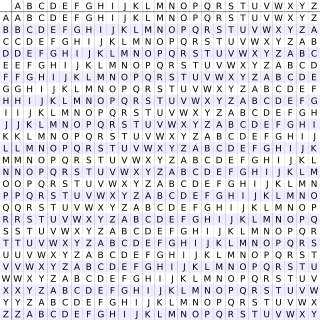
\includegraphics{img/tabularecta.png}
\end{center}

\end{document}
